%% CEUR-WS / DL 2026 format
\documentclass[
% twocolumn,
% hf,
]{ceurart}

\sloppy

%% (DL logo removed for standalone version)

%%% Additional packages
\usepackage{amsmath,amssymb,amsthm}
\usepackage{booktabs}
\usepackage{enumitem}
\usepackage{xcolor}
\usepackage{graphicx}
\usepackage{tikz}
\usetikzlibrary{positioning}

%%% Theorem environments
\newtheorem{theorem}{Theorem}[section]
\newtheorem{lemma}[theorem]{Lemma}
\newtheorem{proposition}[theorem]{Proposition}
\newtheorem{corollary}[theorem]{Corollary}
\theoremstyle{definition}
\newtheorem{definition}[theorem]{Definition}
\newtheorem{examplex}[theorem]{Example}
\newtheorem{remark}[theorem]{Remark}

%%% Notation macros
\newcommand{\ALCI}{\ensuremath{\mathcal{ALCI}}}
\newcommand{\ALC}{\ensuremath{\mathcal{ALC}}}
\newcommand{\ALCIRCC}[1]{\ensuremath{\mathcal{ALCI}_{\mathit{RCC#1}}}}
\newcommand{\LRCC}[1]{\ensuremath{L_{\mathit{RCC#1}}}}
\newcommand{\DR}{\ensuremath{\mathsf{DR}}}
\newcommand{\PO}{\ensuremath{\mathsf{PO}}}
\newcommand{\EQ}{\ensuremath{\mathsf{EQ}}}
\newcommand{\PP}{\ensuremath{\mathsf{PP}}}
\newcommand{\PPI}{\ensuremath{\mathsf{PPI}}}
\newcommand{\TPP}{\ensuremath{\mathsf{TPP}}}
\newcommand{\NTPP}{\ensuremath{\mathsf{NTPP}}}
\newcommand{\TPPI}{\ensuremath{\mathsf{TPPI}}}
\newcommand{\NTPPI}{\ensuremath{\mathsf{NTPPI}}}
\newcommand{\DC}{\ensuremath{\mathsf{DC}}}
\newcommand{\EC}{\ensuremath{\mathsf{EC}}}
\newcommand{\inv}{\ensuremath{\mathsf{inv}}}
\newcommand{\comp}{\ensuremath{\mathsf{comp}}}
\newcommand{\cl}{\ensuremath{\mathsf{cl}}}
\newcommand{\Tp}{\ensuremath{\mathsf{Tp}}}
\newcommand{\Safe}{\ensuremath{\mathsf{Safe}}}
\newcommand{\md}{\ensuremath{\mathsf{md}}}
\newcommand{\Core}{\ensuremath{\mathsf{Core}}}
\newcommand{\Out}{\ensuremath{\mathsf{Out}}}
\newcommand{\Front}{\ensuremath{\mathsf{Front}}}
\newcommand{\EXPTIME}{\textsc{ExpTime}}
\newcommand{\PSPACE}{\textsc{PSpace}}
\newcommand{\naturals}{\mathbb{N}}
\newcommand{\reals}{\mathbb{R}}
\newcommand{\RCCfive}{\{\DR,\PO,\PP,\PPI\}}
%% Round-7 pair-shape / incidence-tag notation
\newcommand{\Q}{\ensuremath{\mathcal Q}}
\newcommand{\U}{\ensuremath{\mathcal U}}
\newcommand{\eqc}{\ensuremath{\approx}}  % equality-port congruence (quotient relation)
\newcommand{\Pos}{\ensuremath{\mathsf{Pos}}}
\newcommand{\Pair}{\ensuremath{\mathsf{Pair}}}
\newcommand{\Tri}{\ensuremath{\mathsf{Tri}}}
\newcommand{\Base}{\ensuremath{\mathsf{B}}}
\newcommand{\lab}{\operatorname{lab}}
\newcommand{\self}{\ensuremath{\mathsf{self}}}
\newcommand{\eqtag}{\ensuremath{\mathsf{eq}}}
\newcommand{\up}{\ensuremath{\mathsf{up}}}
\newcommand{\down}{\ensuremath{\mathsf{down}}}
\newcommand{\side}{\ensuremath{\mathsf{side}}}
\newcommand{\front}{\ensuremath{\mathsf{front}}}
\newcommand{\Eup}{\ensuremath{E_{\uparrow}}}

\begin{document}

%%
%% Rights management information.
\copyrightyear{2026}
\copyrightclause{Copyright for this paper by its authors.
  Use permitted under Creative Commons License Attribution 4.0
  International (CC BY 4.0).}

%%
%% Conference information (removed for standalone version)
%% \conference{DL 2026: 39th International Workshop on Description
%%   Logics, July 17--19, 2026, Lisbon, Portugal}
%% Standalone build guard: ceurart.cls's \maketitle references
%% \ceurConference@name, which only \conference{} defines.  With
%% \conference commented out for the standalone version, define it
%% empty so the paper builds with the bundled class.  Harmless if
%% \conference is later restored (\gdef there overrides this).
\makeatletter
\providecommand\ceurConference@name{}
\makeatother

%%
%% Title
\title{On the Decidability of $\ALCIRCC{5}$:
  A Survey of the Problem, Its History, and a Proposed Solution}
%% PDF/A metadata guard: ceurart.cls writes the XMP \Title as the
%% detokenized \title, so the math macro $\ALCIRCC{5}$ lands literally
%% in the .xmpdata and makes pdfx fail when it re-reads it.  Override
%% the metadata-only title (\casprelimstitle) with a plain-text form;
%% the visible title above is unaffected.
\makeatletter
\csgdef{casprelimstitle}{On the Decidability of ALCI-RCC5: A Survey of the Problem, Its History, and a Proposed Solution}
\makeatother

%%
%% Authors (arXiv candidate: sole human author per arXiv policy;
%% AI-tool contributions are disclosed in the body and in the
%% Declaration on Generative AI below.)
\author[1]{Michael Wessel}[%
email=lambdamikel@gmail.com,
url=https://github.com/lambdamikel,
]
\cormark[1]
\address[1]{LambdaMikel@Home}

\cortext[1]{Corresponding author.}

%%
%% Abstract
\begin{abstract}
The description logic $\ALCIRCC{5}$ extends $\ALCI$ with the five
RCC5 base relations as roles, under composition-table semantics.
Its decidability has been open since Wessel~(2002/2003).
We survey the history of the problem---from Cohn's original proposal
(1993) through Wessel's systematic investigation and Lutz \& Wolter's
related undecidability results (2006)---and explain why all known
undecidability reductions fail for $\ALCIRCC{5}$.
We then present a proposed decision procedure: the \emph{cover-tree
tableau}, which decomposes models into PPI-oriented cover trees
where only $\{\DR,\PO\}$ remain as open cross-edges.
This decomposition, combined with the patchwork property of RCC5,
yields finite blocking via rank-$d$ signatures.
The approach is supported by extensive computational evidence
(911~test concepts, zero mismatches; 775/775~SAT concepts with
cover-tree models) but has not been formally verified by human experts.
We discuss why na\"{\i}ve tableau approaches fail for
$\ALCIRCC{5}$ and how the cover-tree tableau overcomes these obstacles.
\end{abstract}

\begin{keywords}
  description logic \sep
  spatial reasoning \sep
  RCC5 \sep
  decidability \sep
  tableau calculus \sep
  patchwork property
\end{keywords}

\maketitle

%% ====================================================================
\section{Introduction}
\label{sec:intro}
%% ====================================================================

The decidability of concept satisfiability in the spatially extended
description logic $\ALCIRCC{5}$ has been an open problem for over
twenty years.  This paper provides a self-contained overview of the
problem, its intellectual history, the obstacles that have resisted
solution, and a proposed decision procedure that---if correct---would
settle the question positively.

The paper is organized as follows.
Section~\ref{sec:history} traces the history of $\ALCIRCC{5}$
from Cohn's original 1993 proposal through Wessel's systematic
investigation and Lutz \& Wolter's topological undecidability results.
Section~\ref{sec:undecidability} explains why standard undecidability
reductions fail, including a concrete domino-encoding attempt that
we verify is blocked.
Section~\ref{sec:naive-blocking} discusses why na\"{\i}ve tableau
approaches fail for complete-graph logics.
Section~\ref{sec:split-forest} presents the split-forest model
decomposition.
Section~\ref{sec:cover-tree} describes the cover-tree tableau and
explains how it achieves blocking.
Section~\ref{sec:outlook} concludes with an assessment of what
has been achieved and what remains to be done.

\textbf{Disclaimer and AI-tool disclosure.}
This paper was prepared by Michael Wessel with significant
assistance from generative-AI language tools:\@ Claude
(Anthropic, Opus~4.7 and Opus~4.8)~\cite{ClaudeOpus47}, GPT-5.4~Pro
(OpenAI)~\cite{GPT54Pro}, and GPT-5.5~(OpenAI)~\cite{GPT55Repaired}.
The AI tools were used to formalise the mathematical proofs,
implement the cover-tree tableau decision procedure, conduct the
computational verification campaigns, perform the cold reviews
that found successive defects, and draft the manuscript text
including this overview.  Wessel reviewed and edited the content
as needed, directed the research, identified and corrected errors,
and takes full responsibility for the publication's content---including
any errors, mistakes, or misleading statements the AI tools may
have introduced.  See the Declaration on Generative AI at the end
of the paper for further details.  The results and proofs have
\textbf{not been peer-reviewed or verified by human domain
experts}; they are published as a discussion piece, and the one
completeness gap a cold review found (D-1) is repaired at the
manuscript level in round-9 (\S\ref{ssec:round9}) but not
independently certified.  The claims should not be taken as
established results unless independently verified.
Scrutiny, corrections, and feedback are invited.

%% ====================================================================
\section{History of $\ALCIRCC{5}$}
\label{sec:history}
%% ====================================================================

\subsection{Cohn's 1993 proposal}

The idea of combining description logics with qualitative spatial
reasoning via modal accessibility relations was first proposed by
Cohn~\cite{Cohn1993}, who considered treating the RCC8 relations
(or subsets thereof) as modalities in a multi-modal logic.
The framework allowed spatial constraints to be expressed as
modal formulas---e.g., $\langle \PP \rangle C$ for ``some proper
part satisfies~$C$''---but Cohn left all decidability and complexity
questions open.

\subsection{Wessel's $\ALCIRCC{}$ family (2002/2003)}

Wessel~\cite{Wessel2002,Wessel2003,Wessel2001} gave the first rigorous treatment
of the combination, introducing the \emph{$\ALCIRCC{}$ family}:
description logics $\ALCIRCC{k}$ ($k = 1,2,3,5,8$) extending $\ALCI$
with role boxes derived from the RCC composition tables.
In an $\ALCIRCC{k}$ interpretation, every pair of domain elements is
assigned exactly one RCC$k$ base relation, and the composition table
is enforced globally (\emph{strong $\EQ$ semantics}: $\EQ$ is identity).
Models are complete graphs with RCC$k$ edge-colorings.

Wessel established the following:
\begin{itemize}
  \item \textbf{Decidable cases:} $\ALCIRCC{1}$, $\ALCIRCC{2}$,
    and $\ALCIRCC{3}$ are decidable, because their composition
    tables are deterministic or near-deterministic, admitting
    reduction to standard DL techniques.
  \item \textbf{Lower bounds:} $\ALCIRCC{5}$ is $\PSPACE$-hard;
    $\ALCIRCC{8}$ is $\EXPTIME$-hard.
  \item \textbf{Open:} The decidability of $\ALCIRCC{5}$ and
    $\ALCIRCC{8}$ was left as the central open problem.
\end{itemize}

In a series of companion reports, Wessel also mapped out the
decidability landscape for description logics with general
composition-based role inclusion axioms:
\begin{itemize}
  \item $\ALC_{\mathcal{RA}}$ (arbitrary role axioms) is
    \textbf{undecidable}, via reduction from the Post
    Correspondence Problem~\cite{Wessel2001RA}.
  \item $\ALC_{\mathcal{RA}}^\ominus$ (non-disjoint-roles
    variant) is also \textbf{undecidable}, via reduction from
    non-empty CFG intersection~\cite{Wessel2000RA}.
  \item $\ALC_{\mathcal{RA}_{SG}}$ (admissible role boxes:
    deterministic, functional, complete, and associative) is
    \textbf{decidable} (\EXPTIME-complete, via reduction to
    $\ALC$ with general TBoxes)~\cite{Wessel2000SG}; adding
    unqualified number restrictions ($\mathcal{ALCN}_{\mathcal{RA}_{SG}}$)
    makes it undecidable again.
\end{itemize}
$\ALCIRCC{5}$ sits precisely in the gap: its role box is
non-deterministic (unlike $\ALC_{\mathcal{RA}_{SG}}$) but
has the patchwork property (unlike
$\ALC_{\mathcal{RA}}/\ALC_{\mathcal{RA}}^\ominus$).

\begin{remark}[Key difficulties]
$\ALCIRCC{5}$ has none of the properties that standard DL
decidability proofs rely on:
(i)~no tree model property (models are complete graphs),
(ii)~no finite model property (some satisfiable concepts require
infinite models),
(iii)~a non-deterministic role box (multi-valued composition entries).
\end{remark}

For reference, the full RCC5 composition table is given in
Table~\ref{tab:comp}.  Reading: row = $S(b,c)$, column = $R(a,b)$,
entry = possible relations for $(a,c)$.

\begin{table}[ht]
\centering
\caption{The RCC5 composition table ($*$ = all five relations).}
\label{tab:comp}
\renewcommand{\arraystretch}{1.15}
\begin{tabular}{l|ccccc}
\toprule
$\comp$ & $\DR(a,b)$ & $\PO(a,b)$ & $\EQ(a,b)$ & $\PPI(a,b)$ & $\PP(a,b)$ \\
\midrule
$\DR(b,c)$ & $*$ & $\DR,\PO,\PPI$ & $\DR$ & $\DR,\PO,\PPI$ & $\DR$ \\
$\PO(b,c)$ & $\DR,\PO,\PP$ & $*$ & $\PO$ & $\PO,\PPI$ & $\DR,\PO,\PP$ \\
$\EQ(b,c)$ & $\DR$ & $\PO$ & $\EQ$ & $\PPI$ & $\PP$ \\
$\PP(b,c)$ & $\DR,\PO,\PP$ & $\PO,\PP$ & $\PP$ & $\PO,\EQ,\PP,\PPI$ & $\PP$ \\
$\PPI(b,c)$ & $\DR$ & $\DR,\PO,\PPI$ & $\PPI$ & $\PPI$ & $*$ \\
\bottomrule
\end{tabular}
\end{table}

\noindent
Key composition facts exploited in the cover-tree theory
(Sections~\ref{sec:split-forest}--\ref{sec:cover-tree}):
$\comp(\PP,\DR) = \{\DR\}$ and $\comp(\DR,\PPI) = \{\DR\}$
(DR rigidity);
$\comp(\PP,\PP) = \{\PP\}$ and $\comp(\PPI,\PPI) = \{\PPI\}$
(transitivity);
and $\comp(\DR,\PO) = \{\DR,\PO,\PP\}$
(PP can be \emph{forced} by composition and universal filtering;
see Example~\ref{ex:pp-forcing}).

\subsection{Wessel's grid constructions and the coincidence obstruction}
\label{sec:wessel-grid}

In his investigation of $\ALCIRCC{8}$~\cite{Wessel2003}, Wessel
made two important discoveries:

\medskip\noindent\textbf{1.\ Even-odd chains (Section~4.4.2).}
The $\TPP/\NTPP$ distinction in RCC8 allows the construction of
\emph{functional successor chains}: each node alternates between
$\mathit{even}$ and $\mathit{odd}$, and a node can distinguish its
direct $\TPPI$-successor from all indirect ones by parity.
Wessel used this to encode a binary $n$-bit counter, proving
$\ALCIRCC{8}$ is $\EXPTIME$-hard.

\medskip\noindent\textbf{2.\ The grid coincidence obstruction (Section~4.4.3,
Figure~11).}
Wessel constructed explicit RCC8 networks isomorphic to
$n \times n$ grids, using $\TPP$ for horizontal and vertical
successors.  However, he identified a fundamental obstacle to
encoding domino tilings: the \emph{coincidence condition}
$R_X \circ R_Y = R_Y \circ R_X$ (east-of-north equals
north-of-east) cannot be enforced by concept terms.
The composition table allows $\{PO, EQ, TPP, NTPP, TPPI, NTPPI\}$
at the coincidence point---too many options.  Wessel concluded:
\begin{quote}
``Even though these infinite models do exist, we have found no way
to \emph{enforce} the depicted model(s) by means of a concept term.''
\end{quote}
Wessel further observed that adding a hybrid logic binding operator
$\downarrow$ (nominals) would immediately yield undecidability,
confirming that the coincidence condition is the \emph{precise
boundary}.

Wessel thus independently developed, three to four years before
Lutz--Wolter, the RCC8 description-logic analogues of these
ingredients---the even-odd chain, an explicit two-dimensional
$\TPP/\NTPP$ grid, and the first identification of the coincidence
gap as the decisive obstacle.  Lutz--Wolter later obtained
undecidability by a \emph{different} route---a linearized tiling
enumeration (their~\S5, following Marx--Reynolds) that sidesteps the
two-dimensional coincidence rather than enforcing it---so this is
shared lineage and prior identification, not a dependence of their
proof on Wessel's constructions.

\subsection{Lutz \& Wolter (2006)}

Lutz and Wolter~\cite{LutzWolter2006} studied \emph{modal logics
of topological relations}, denoted $\LRCC{8}$, $\LRCC{5}$, etc.
These have the same \emph{syntax} as $\ALCIRCC{}$ but are
interpreted over \emph{topological models}: the domain elements
are regular closed subsets of a topological space (typically~$\reals^n$).
They proved:
\begin{itemize}
  \item $\LRCC{8}$ is \textbf{undecidable} (their~\S5: a linearized
    $\NTPP$-chain enumeration of tile positions, following
    Marx--Reynolds, whose faithfulness relies on the geometry of
    $\reals^n$; no two-dimensional grid coincidence is enforced).
  \item $\LRCC{5}(\mathit{RS}^\exists)$ is \textbf{undecidable}
    (reduction from $S5^3$ via supremum regions).
  \item $\LRCC{5}(\mathit{RS})$ is \textbf{open}. Lutz and Wolter
    explicitly wrote (p.~31): ``Perhaps the most interesting
    candidate is $L_{RCC5}(RS)$ [\ldots] to which the reduction
    exhibited in Section~8 does not apply.''
\end{itemize}

The logic $\ALCIRCC{5}$ is exactly $\LRCC{5}(\mathit{RS})$:
arbitrary complete-graph models with composition-table semantics.
The problem has been recognized as open by leading researchers
since 2006.

%% ====================================================================
\section{Why Undecidability Reductions Fail}
\label{sec:undecidability}
%% ====================================================================

Undecidability proofs for description logics use a variety of
techniques: grid encoding ($\naturals \times \naturals$ domino
tiling, requiring functional roles or number restrictions),
reduction from the Post Correspondence Problem (PCP), reduction
from context-free grammar (CFG) intersection, or simulation of
$S5^3$ via geometric constructions.
$\ALCIRCC{5}$ lacks the features that each of these techniques
exploits: it has no functional roles, no number restrictions,
no arbitrary role box, and no geometric coincidence conditions.

\subsection{Blocked reduction routes}

\begin{table}[t]
\caption{Why standard undecidability reductions fail for $\ALCIRCC{5}$.}
\label{tab:blocked}
\begin{tabular}{p{3.0cm}p{3.8cm}p{3.5cm}}
\toprule
\textbf{Source Problem} & \textbf{Technique} & \textbf{Missing in $\ALCIRCC{5}$} \\
\midrule
$\naturals \times \naturals$ domino & Graded modalities + transitivity & Number restrictions \\
$\ALC_{\mathcal{RA}}$ \cite{Wessel2001RA} & Post Correspondence Problem & Arbitrary role axioms \\
$\ALC_{\mathcal{RA}}^\ominus$ \cite{Wessel2000RA} & Non-empty CFG intersection & Non-disjoint roles \\
$\ALCIRCC{8}$ (Wessel) & Grid via $\TPP/\NTPP$ & $\TPP/\NTPP$ distinction \\
$\LRCC{8}$ (Lutz--Wolter) & Linearized topological enumeration & Topological rigidity \\
$\LRCC{5}(\mathit{RS}^\exists)$ & $S5^3$ via supremum regions & Supremum closure \\
\bottomrule
\end{tabular}
\end{table}

Table~\ref{tab:blocked} summarizes the blocked routes.
The \textbf{patchwork property} of RCC5 (Renz \& Nebel~\cite{RenzNebel1999})---local
(triple-wise) consistency implies global consistency for atomic
networks---actively resists grid encoding, since tiling reductions
require rigid global constraints that go beyond local consistency.

\subsection{A concrete domino attempt in $\ALCIRCC{5}$}
\label{sec:domino-attempt}

Can we encode a domino-like grid using $\PP/\PPI$ chains in RCC5?
Consider the concept:
\begin{align*}
  X \;=\; &\exists\PPI.\exists\PPI.C \;\sqcap\; \exists\PPI.\exists\PPI.D \\
  &\sqcap\; \forall\PPI.\forall\PPI.(\forall\PO.(\neg C \sqcap \neg D)
    \sqcap \forall\DR.(\neg C \sqcap \neg D) \\
  &\qquad\qquad\qquad\quad\;\;
    \sqcap\; \forall\PPI.(\neg C \sqcap \neg D)
    \sqcap \forall\PP.(\neg C \sqcap \neg D)) \\
  &\sqcap\; \forall\PPI.\exists\PPI.X
\end{align*}
The intent: each $X$-node has two $\PPI$-grandchildren colored $C$
and $D$ (the ``square''), and the universals isolate the colored
nodes from all non-$\EQ$ neighbors.  The recursive
$\forall\PPI.\exists\PPI.X$ forces infinite repetition.

\medskip\noindent\textbf{One level is satisfiable.}
Without the recursive conjunct, $X$ has a 3-element model:
$z \;\PP\; y \;\PP\; x$, with $z \in C \sqcap D$.
The two grandchildren are forced to be \emph{the same element}
($\EQ$ collapse): if $z_1 \neq z_2$, they would be related by
some $R \in \RCCfive$, and the universals would require $z_2 \notin D$
(firing $z_1$'s $\forall R.\neg C \sqcap \neg D$).
So $z_1 = z_2 \in C \sqcap D$, and the universals are vacuously
satisfied (the only neighbors of~$z$ are PP-predecessors, not
PO/DR/PPI-neighbors).

\medskip\noindent\textbf{Two levels is unsatisfiable.}
Adding $\forall\PPI.X$: the $\PPI$-child $y$ must itself satisfy~$X$
(without recursion), producing a new $C \sqcap D$-labeled element~$w$
as a $\PPI$-child of~$z$.  But $z$ is a $\PPI$-grandchild of~$x$,
and $x$'s universals fire: $z$'s $\PPI$-neighbor~$w$ must satisfy
$\neg C \sqcap \neg D$.  Yet $w \in C \sqcap D$.
\textbf{Contradiction.}

This was verified computationally: a simplified version
$X_1 = \exists\PPI.\exists\PPI.C \sqcap \forall\PPI^3.\neg C$
is SAT; $X_2 = X_1 \sqcap \forall\PPI.X_1$ is UNSAT.
The domino encoding collapses at depth~2 because the isolation
constraints from the grandparent level kill the colored elements
created by the recursive unfolding.

\begin{remark}
The failure is not accidental.  In $\ALCIRCC{5}$, the only way to
create ``functional'' successors is via $\PP/\PPI$ chains, but
$\comp(\PPI,\PPI) = \{\PPI\}$ makes these chains
\emph{transitive}---grandparent universals automatically propagate
to grandchildren, preventing the positional diversity needed for
grid encoding.  In $\ALCIRCC{8}$, the $\TPP/\NTPP$ distinction
breaks this transitivity (a direct $\TPPI$-child is distinguishable
from indirect descendants), which is why Wessel's even-odd chain
works there but has no RCC5 analogue.
\end{remark}

\subsection{A concrete domino attempt in $\ALCIRCC{8}$}
\label{sec:domino-attempt-rcc8}

The remark above suggests the $\TPPI/\NTPPI$ distinction in
$\ALCIRCC{8}$ might rescue the construction: a direct successor
($\TPPI$) and an indirect one ($\NTPPI$) are genuinely
distinguishable, so perhaps the level-2 collapse can be avoided.
We attempt the analogue and show that while it escapes the RCC5
failure mode, it fails for a different reason---Wessel's
\emph{coincidence obstruction}~\cite{Wessel2003}.

\medskip\noindent\textbf{The schema.} Let $\textsf{Corner}$ be the
concept that isolates a node from all non-$\EQ$ neighbors:
\[
  \textsf{Corner} \;=\;
  \bigwedge_{R \,\in\, \{\DC,\EC,\PO,\TPP,\NTPP,\TPPI,\NTPPI\}}
    \forall R.(\neg C \sqcap \neg D).
\]
The isolation is placed \emph{locally on the colored grandchildren}
rather than as an ancestral $\forall\TPPI.\forall\TPPI$ universal,
so it cannot propagate transitively through the recursion:
\begin{align*}
  X \;=\; &\exists\TPPI.\exists\TPPI.(C \sqcap \textsf{Corner})
    \;\sqcap\; \exists\TPPI.\exists\TPPI.(D \sqcap \textsf{Corner}) \\
  &\sqcap\; \forall\TPPI.(\neg C \sqcap \neg D)
    \;\sqcap\; \forall\TPPI.X.
\end{align*}
The third conjunct $\forall\TPPI.(\neg C \sqcap \neg D)$ forces the
corner relation $x \to z$ to be $\NTPPI$ (not $\TPPI$), using
$\comp(\TPPI,\TPPI) = \{\TPPI, \NTPPI\}$.

\medskip\noindent\textbf{Level 1 is satisfiable, with a real
direct/indirect distinction.} Without recursion, $x$ has
$\TPPI$-children $y_1, y_2$ (the two ``direct'' positions) and a
single corner $z$ reached by $\TPPI$-$\TPPI$ chains from both
$y_1$ and $y_2$.  The EQ-collapse at level~2 works exactly as
in RCC5: $z_1 \in C \sqcap \textsf{Corner}$ and $z_2 \in D \sqcap
\textsf{Corner}$ are mutual non-$\EQ$ neighbors only if
$\textsf{Corner}$ is violated, so under strong-$\EQ$ semantics
$z_1 = z_2 = z$.  Crucially, $z \neq y_1, y_2$ in general: $z$ is
$\NTPPI$ of $x$ while $y_1, y_2$ are $\TPPI$---the direct/indirect
distinction survives, which is a genuine RCC8 refinement over the
RCC5 attempt of~\S\ref{sec:domino-attempt}.

\medskip\noindent\textbf{Level 2 collapses via the coincidence
obstruction.} Adding $\forall\TPPI.X$: the $\TPPI$-child $y$ of
$x$ satisfies $X$, producing its own corner $w \in C \sqcap D
\sqcap \textsf{Corner}$ at $\NTPPI$-distance from $y$, and hence
at $\NTPPI$-distance from $x$ via
$\comp(\TPPI, \NTPPI) = \{\NTPPI\}$.  Now $x$'s own corner $z$ and
$y$'s corner $w$ are distinct grid positions in the intended
reading---but as elements of the model they are related by some
RCC8 base relation.  Since $z$ carries $\textsf{Corner}$, every
non-$\EQ$ neighbor of $z$ lies in $\neg C \sqcap \neg D$.  But
$w \in C \sqcap D$.  Therefore $z = w$ under strong-$\EQ$.
\textbf{All corners across the grid coincide at a single point.}

\medskip\noindent\textbf{Why the $\TPPI/\NTPPI$ trick fails.} In
the RCC5 attempt the collapse is a \emph{transitive-propagation}
failure: the grandparent universal fires on great-grandchildren
because $\comp(\PPI,\PPI) = \{\PPI\}$.  Moving the isolation to a
local $\textsf{Corner}$ marker and using the non-transitive piece
$\comp(\TPPI,\TPPI) = \{\TPPI, \NTPPI\}$ eliminates that specific
pathway---the universal at the grandparent no longer reaches
deeper nodes.  But a \emph{different} obstruction takes over: the
composition table permits any of
$\{\PO, \EQ, \TPP, \NTPP, \TPPI, \NTPPI\}$ between two corners at
different intended grid coordinates, and nothing in the concept
language rules out $\EQ$.  The $\textsf{Corner}$ markers themselves
then force the EQ-merge.  This is exactly the obstruction Wessel
identified in report7.pdf, Figure~11 (cf.~\S\ref{sec:wessel-grid}):
the composition table does not carry the rigidity needed to keep
distinct grid cells distinct.

\begin{remark}
The failure mode is structurally different from the RCC5 one but
traces back to the same root cause.  Lutz--Wolter's $\LRCC{8}$
reduction \emph{circumvents} the coincidence obstruction rather than
enforcing it: they linearize the plane into a single $\NTPP$-chain
(the Marx--Reynolds enumeration) and recover the vertical direction
from the enumeration, so no ``north-of-east $=$ east-of-north''
coincidence has to be forced; the geometry of $\reals^n$ only has to
keep that linear encoding faithful~\cite{LutzWolter2006}.  No such rigidity is available in
the abstract RCC8 semantics of $\ALCIRCC{8}$: a pure composition
table allows corner points to merge freely, and the $\TPPI/\NTPPI$
distinction---while useful locally for a direct/indirect
separation at level~2---cannot be chained to enforce an unbounded
$\naturals \times \naturals$ grid.  This matches the open-problem
status of $\ALCIRCC{8}$ decidability noted in~\cite{LutzWolter2006}
and further discussed in~\cite{Wessel2003}.
\end{remark}

%% ====================================================================
\section{Why Na\"{\i}ve Tableau Blocking Fails}
\label{sec:naive-blocking}
%% ====================================================================

Standard DL tableau calculi achieve termination through
\emph{blocking}: if a node~$x$ has the same label as an ancestor~$y$,
we can reuse $y$'s subtree for~$x$, cutting off infinite
branches.  The key requirement is that the ``reuse'' preserves
all constraints---in tree-shaped models, a blocked node's
interactions are limited to its parent edge, so label equality suffices.

In $\ALCIRCC{5}$, models are \emph{complete graphs}: every pair
of domain elements is related by an RCC5 base relation.
A node interacts not just with its parent and children, but with
\emph{every other node in the model}.
This creates a fundamental obstacle for blocking.

\begin{examplex}[Blocking breaks with cross-edges]
\label{ex:blocking-fail}
Consider $C_0 = \exists\PPI.A \sqcap \exists\DR.\neg A
\sqcap \exists\PO.\top$.
A tableau might generate nodes:
\begin{itemize}[nosep]
  \item $x_0$: root, satisfies $C_0$
  \item $x_1$: $\PPI$-child of $x_0$, type contains $A$
  \item $x_2$: $\DR$-witness for $x_0$, type contains $\neg A$
\end{itemize}
Now $x_1$ and $x_2$ must be related by some RCC5 relation~$R$,
and $R$ must be safe for their types.  If $x_1$ generates a
descendant $x_3$ with the same label as $x_1$, na\"{\i}ve blocking
would declare $x_3$ blocked.  But $x_3$'s relation to~$x_2$ may
differ from $x_1$'s relation to~$x_2$: via composition,
$\comp(\inv(\PPI), \DR) = \comp(\PP, \DR) = \{\DR\}$ forces
$x_1$ to be $\DR$-related to~$x_2$, while $x_3$ (deeper in the
tree) may face a different forced relation.  The blocked node's
cross-edge commitments differ from the blocking node's.
\end{examplex}

Multiple sophisticated blocking strategies have been tried and
failed for $\ALCIRCC{5}$~\cite{ALCIRCC5Outdated,StatusAfterFW,ResponseGPTBlocking}:
\begin{enumerate}
  \item \textbf{Profile-cached blocking} (GPT-5.4)~\cite{ResponseGPTBlocking}: Caches
    ``coherent predecessor blocks'' to compare global neighborhoods.
    Fails because the \emph{color structure changes during
    unraveling}---when a blocked subtree is replayed, the
    edge-coloring to nodes outside the subtree is not preserved.
  \item \textbf{Meet-semilattice replay} (GPT-5.4)~\cite{ResponseGPTBlocking}: Uses a
    meet-semilattice structure on labels to ensure robust
    normalization.  Same unraveling gap.
  \item \textbf{Tri-neighborhood blocking} (Claude)~\cite{TriangleBlocking}: Matches not
    just node labels but entire \emph{triangle neighborhoods}
    (the set of all types of 2-element subsets involving the node).
    \textbf{Termination disproved}: frontier nodes continuously
    acquire new triangle types as new neighbors are added, so
    $\mathrm{Tri}(x) \subsetneq \mathrm{Tri}(y)$ for frontier~$x$
    and interior~$y$---blocking never triggers.
  \item \textbf{Finite-witness / patchwork-augmentation probes}
    (Claude)~\cite{FWProof,PatchworkAugmentation,TypedPatchworkCounterexample}:
    Probes of a finite-witness conjecture and typed-patchwork
    augmentations for the contextual tableau, both refuted by
    explicit counterexamples.
\end{enumerate}

The common obstacle is the \textbf{blocking dilemma}: making the
blocking condition strong enough for soundness (matching all
cross-edge interactions) prevents termination (the cross-edge
context keeps growing), and vice versa.  A full catalogue of
retracted approaches is maintained
in~\cite{ALCIRCC5Outdated}; the overall project is summarised at
the repository~\cite{ALCIRCC5Repo}.

%% ====================================================================
\section{Split-Forest Model Decomposition}
\label{sec:split-forest}
%% ====================================================================

The breakthrough insight, due to Wessel, is to decompose
$\ALCIRCC{5}$ models into a \emph{tree layer} and a
\emph{cross-edge layer}, where the cross-edge layer is simple
enough to handle without full global blocking.
Figure~\ref{fig:whiteboard} reproduces the original whiteboard
sketch from April~7, 2026:\@ $\PPI$ chains form trees, $\DR/\PO$
are sibling cross-edges, and $\DR$ propagates rigidly downward
along $\PP$-chains.

\begin{figure}[ht]
\centering
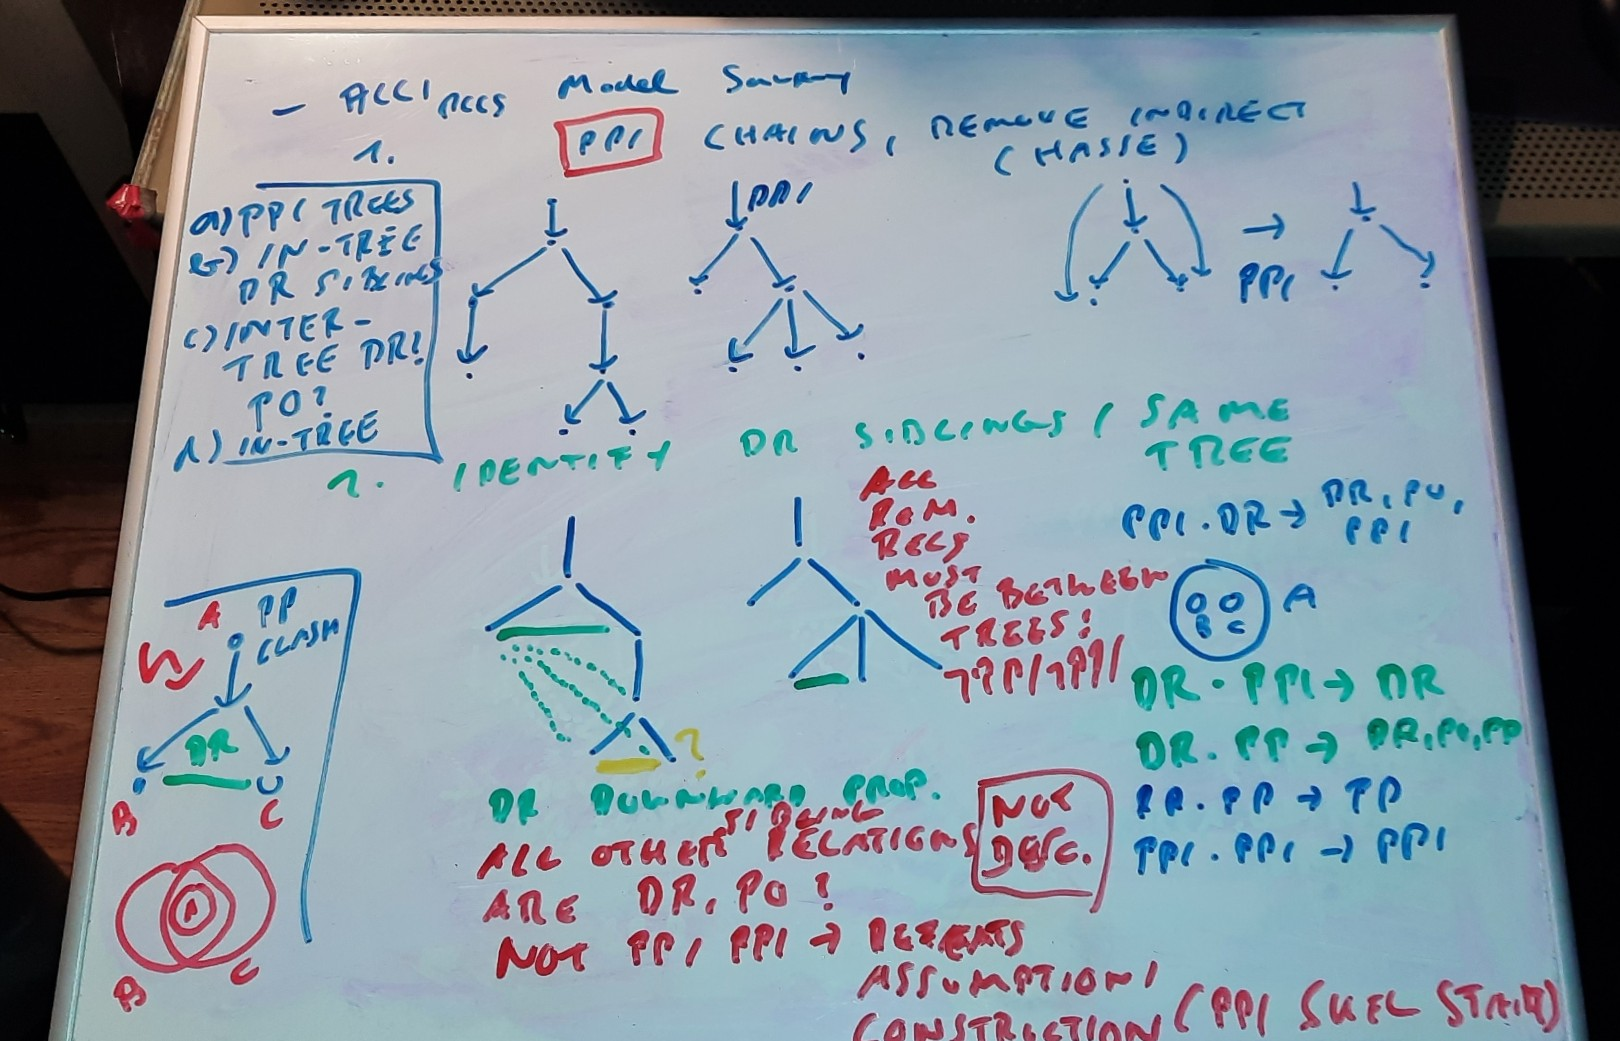
\includegraphics[width=0.85\columnwidth]{20260407_062616.jpg}
\caption{Wessel's whiteboard sketch (April~7, 2026) of the
  split-forest decomposition for $\ALCIRCC{5}$.  Vertical
  $\PPI$-chains form the cover-tree backbone (with join nodes
  split into $\EQ$-mates); $\DR/\PO$ become sibling cross-edges
  between non-comparable subtrees; and $\DR$ propagates rigidly
  downward because $\comp(\PP,\DR)=\comp(\DR,\PPI)=\{\DR\}$, so
  the residual cross-edge alphabet is just $\{\DR,\PO\}$, which
  is trivially arc-consistent.  Every subsequent formalisation
  in this paper---GPT-5.4's split-forest semantics, Claude's
  cover-tree tableau, and GPT-5.5's round-7-through-round-9
  sketches---rests on this two-layer decomposition.}
\label{fig:whiteboard}
\end{figure}

\subsection{Cover trees}

In any $\ALCIRCC{5}$ model, the $\PP/\PPI$ relation is a
strict partial order (by composition: $\comp(\PP,\PP) = \{\PP\}$).
Orient this order downward ($\PPI$ = ``has proper part'') to
obtain a DAG.  If the DAG has join nodes (elements with multiple
$\PP$-predecessors), split them into $\EQ$-copies, one per parent
path.  The result is a rooted forest---the \emph{cover tree}.

\begin{definition}[Cover tree]
A \emph{cover-tree presentation} of an $\ALCIRCC{5}$ model
$\mathcal{I}$ is a rooted tree $T$ with a surjection
$\mathrm{orig}: T \to \Delta^{\mathcal{I}}$ such that:
(i) $u$ is the parent of $v$ in $T$ iff
$\mathrm{orig}(u) \;\PPI\; \mathrm{orig}(v)$ (immediate containment),
and (ii) tree nodes mapping to the same element are $\EQ$-mates
(weak-$\EQ$ semantics, convertible to strong-$\EQ$ by typed
congruence quotient).
\end{definition}

\subsection{The key observation: DR rigidity}

In the cover tree, what relations can hold between nodes in
different sibling subtrees?  Consider sibling roots $s$ and $t$
(children of the same parent), and elements $x$ below~$s$, $y$
below~$t$ in the tree.
An element~$x$ below~$s$ is in the \emph{$\Core$} of the sibling
pair $(s,t)$ if $\mathrm{orig}(x)$ is a common descendant of both
$\mathrm{orig}(s)$ and $\mathrm{orig}(t)$ in the original model's
$\PP$ order---i.e., $\mathrm{orig}(x)$ is a proper part of both.
Core elements are handled by $\EQ$-splitting; the interesting
question concerns non-$\Core$ elements.

\begin{proposition}[Wessel]
\label{prop:dr-rigid}
After $\EQ$-splitting, only $\DR$ and $\PO$ are possible between
non-$\Core$ elements of sibling subtrees.
\end{proposition}

\begin{proof}
\begin{itemize}[nosep]
  \item $\EQ(x,y)$: In the original DAG (before splitting),
    $x = y$ would mean a single element is a $\PP$-descendant of
    both $s$ and $t$---i.e., it is in the $\Core$.
    After splitting, this element is duplicated into
    distinct tree nodes $x'$ below~$s$ and $y'$ below~$t$,
    with $\mathrm{orig}(x') = \mathrm{orig}(y')$
    ($\EQ$-mates in the weak-$\EQ$ presentation).
    Since $x' \neq y'$ as tree nodes, $\EQ(x',y')$ is
    impossible under strong $\EQ$ semantics.
  \item $\PP(x,y)$: would mean $x$ lies below $y$ in the part-of
    order, hence below~$t$, making $x$ a common descendant
    ($\Core$).
  \item $\PPI(x,y)$: would place $y$ below~$x$ below~$s$, meaning
    $t$ lies below $s$---contradicting sibling incomparability.
\end{itemize}
Only $\DR$ and $\PO$ remain.  Furthermore, $\DR$ propagates
rigidly: $\comp(\PP, \DR) = \{\DR\}$ and $\comp(\DR, \PPI) = \{\DR\}$,
so if $s \;\DR\; t$, then \emph{every} descendant of~$s$ is $\DR$
to~$t$ and all its descendants.
\end{proof}

\subsection{Trivial arc-consistency of $\{\DR,\PO\}$ networks}

The consequence of Proposition~\ref{prop:dr-rigid} is that the
cross-edge constraint network uses only $\{\DR, \PO\}$ as possible
relations (plus $\{\DR\}$ for $\DR$-rigid pairs).

\begin{proposition}
\label{prop:drpo-arc}
For all $R, S \in \{\DR, \PO\}$:
$\comp(R, S) \cap \{\DR, \PO\} \neq \varnothing$.
\end{proposition}

This means a $\{\DR,\PO\}$ disjunctive network is
\emph{trivially arc-consistent}: every domain is either
$\{\DR\}$, $\{\PO\}$, or $\{\DR,\PO\}$, and composing any two
non-empty domains produces a non-empty result.
By the patchwork property~\cite{RenzNebel1999}, the network
therefore has a globally consistent atomic refinement whenever
every domain is non-empty.

This is the central simplification: \emph{checking that each type
pair has a non-empty $\{\DR,\PO\}$-safe set suffices for
cross-edge consistency.}  No full path-consistency computation is
needed.

%% ====================================================================
\section{The Cover-Tree Tableau}
\label{sec:cover-tree}
%% ====================================================================

\subsection{Algorithm overview}

The cover-tree tableau searches for a \emph{valid type set}:
a finite set $T \subseteq \Tp(C_0)$ of Hintikka types that
contains a root type realizing~$C_0$ and satisfies four conditions:

\begin{enumerate}[label=(CT\arabic*)]
  \item \textbf{Demand closure}: every existential demand
    $\exists R.D$ in every $\tau_i \in T$ has an $R$-safe
    witness $\tau_j \in T$ with $D \in \tau_j$.
  \item \textbf{Cross-edge consistency}: every pair
    $\tau_i, \tau_j \in T$ has either $\Safe(\tau_i,\tau_j)
    \cap \{\PP,\PPI\} \neq \varnothing$ (tree-relatable) or
    $\Safe(\tau_i,\tau_j) \cap \{\DR,\PO\} \neq \varnothing$
    (cross-relatable).
  \item \textbf{Cover-tree sibling compatibility}: for each
    type $\tau_i$ with multiple $\DR/\PO$ demands, the witnesses
    can be jointly assigned such that every witness pair satisfies
    $\comp(\inv(R_m), R_{m'}) \cap \{\DR,\PO\} \cap
    \Safe_{\DR/\PO}(\tau_{j_m}, \tau_{j_{m'}}) \neq \varnothing$.
  \item \textbf{Composition propagation}: for each type with
    multiple demands of \emph{any} role combination, witnesses
    $\tau_{j_1}, \tau_{j_2}$ must satisfy
    $\comp(\inv(R_1), R_2) \cap \Safe(\tau_{j_1}, \tau_{j_2})
    \neq \varnothing$.
\end{enumerate}

The algorithm terminates because $|\Tp(C_0)| \leq 2^{|\cl(C_0)|}$
is finite, and the type set grows monotonically during the search.

\subsection{How blocking works}

The crucial difference from na\"{\i}ve tableau approaches is the
\emph{separation of layers}:

\begin{itemize}
  \item The \textbf{tree layer} ($\PP/\PPI$) handles
    ancestor/descendant demands.  Since $\PP/\PPI$ form a tree,
    standard tree-model arguments apply: blocking via
    \emph{rank-$d$ signatures} (the type information visible
    within modal depth~$d = \md(C_0)$) yields a finite
    representation.

  \item The \textbf{cross layer} ($\DR/\PO$) handles demands for
    disconnected or partially overlapping regions.  Because the
    cross-edge network uses only $\{\DR,\PO\}$---which is
    trivially arc-consistent---the cross-layer check reduces to a
    simple pairwise non-emptiness condition (CT2), not a global
    consistency computation.
\end{itemize}

Na\"{\i}ve blocking fails because it tries to handle both layers
simultaneously: the tree structure provides natural blocking, but
the cross-edges to distant nodes keep changing, preventing a match.
The cover-tree tableau sidesteps this by \emph{not} blocking on
cross-edge context---instead, it verifies cross-edge consistency
as a separate, global check on the finite type set.

\begin{examplex}[A concept that defeats na\"{\i}ve blocking but
  works with cover trees]
\label{ex:cover-tree-win}
Consider $C_0 = \exists\PO.A \sqcap \exists\PP.\neg B \sqcap
\forall\DR.A$.
In a na\"{\i}ve tableau, the $\PP$-child needs further expansion;
blocking requires matching both the label \emph{and} the
triangle neighborhood (relations to the $\PO$-witness and all
other nodes).  Since the $\PO$-witness forces $\DR$-relations
to the $\PP$-child's subtree (via $\comp(\PO, \PP) = \{\DR,\PO,\PP\}$),
the cross-edge context keeps evolving.

In the cover-tree tableau: the $\PP$-witness is an ancestor in
the tree, the $\PO$-witness is a cross-edge in a sibling subtree.
The $\forall\DR.A$ fires only on $\DR$-related nodes---the
ancestor is $\PP$-related (not $\DR$), so no conflict.
The type set $T$ needs a type for the root (containing $C_0$),
one for the $\PO$-witness (containing $A$), and one for the
$\PP$-witness (containing $\neg B$).  Cross-edge consistency
(CT2) checks that every pair has a non-empty safe set in
$\{\DR,\PO\}$---a one-time pairwise check, not an evolving
context.
\end{examplex}

\begin{examplex}[Implicit PP via composition forcing]
\label{ex:pp-forcing}
The concept
\[
  X \;=\; \exists\DR.\exists\PO.C
    \;\sqcap\; \forall\DR.\neg C
    \;\sqcap\; \forall\PO.\neg C
    \;\sqcap\; \forall\PP.X
\]
contains no $\exists\PP$ demand, yet it requires an infinite
model with forced $\PP$ edges.

A node~$r$ satisfying~$X$ has a $\DR$-neighbor~$a$
(with $\exists\PO.C$) and $a$'s $\PO$-neighbor~$b$
(with~$C$).  By Table~\ref{tab:comp}, the relation
between $r$ and $b$ lies in
$\comp(\DR,\PO) = \{\DR,\PO,\PP\}$.
But $r$ has $\forall\DR.\neg C$ and $\forall\PO.\neg C$,
and $b \in C$---so $\DR$ and $\PO$ are blocked, leaving
\emph{only}~$\PP$.  The $\PP$ edge is \textbf{forced} by
composition plus universal filtering, with no explicit
$\exists\PP$ in the concept.

Since $r \;\PP\; b$, node $b$ is an \emph{ancestor} of~$r$
in the cover tree.  The recursive $\forall\PP.X$ forces $b$
to also satisfy~$X$, creating its own
$\DR \to \PO$ chain and forcing yet another $\PP$-ancestor
above it:
\[
  r \;\PP\; b \;\PP\; b' \;\PP\; b'' \;\PP\; \cdots
\]
The model is necessarily infinite.  The cover-tree tableau
handles this finitely: the type for $C$-elements can serve as
its own $\PP$-ancestor (different domain elements, same
abstract state), so a three-element type set
$\{\tau_0(C,X),\; \tau_1(\neg C, \exists\PO.C),\;
  \tau_2(\neg C, \text{root})\}$
represents the infinite model.

This pattern---$\PP$ edges arising purely from composition and
universal filtering---is a distinctive feature of $\ALCIRCC{5}$
and illustrates why the complete-graph semantics require careful
handling of implicit spatial constraints.
\end{examplex}

\begin{examplex}[The ``$\PO$-loop'': 2-element SAT via symmetric cycles]
\label{ex:po-loop}
Naive reasoning suggests
\[
  Y \;=\; C
    \;\sqcap\; \exists\PO.\exists\PO.C
    \;\sqcap\; \forall\PO.\neg C
    \;\sqcap\; \forall\DR.\neg C
    \;\sqcap\; \forall\PP.\neg C
    \;\sqcap\; \forall\PPI.\neg C
\]
should be unsatisfiable: any witness chain
$d \;\PO\; a \;\PO\; b$ with $b \in C$ needs
$\rho(d,b) \in \comp(\PO,\PO) = \{\DR,\PO,\PP,\PPI,\EQ\}$,
and the four universals $\forall R.\neg C$ seem to block every
non-$\EQ$ option (each forces $b \in \neg C$, yet $b \in C$).

But $Y$ is in fact \textbf{satisfiable}, via the two-element model
$\{d,a\}$ with $C^{\mathcal I} = \{d\}$ and $\rho(d,a) = \PO$.
Because $\PO$ is symmetric
($\PO(d,a) \Rightarrow \PO(a,d)$), the chain
$d \;\PO\; a \;\PO\; d$ loops back to the root itself: the
``third node'' of the $\exists\PO.\exists\PO$ formula \emph{is}
$d$, under strong $\EQ$ identity. Two syntactic positions in the
nested existential map to the same semantic element.

The universals $\forall R.\neg C$ constrain $d$'s \emph{outgoing}
$R$-neighbours (the sole $\PO$-neighbour $a \in \neg C$
satisfies them), but they do \textbf{not} prevent $d$ from
\emph{being} a $\PO$-neighbour of $a$: the witness for $a$'s
$\exists\PO.C$ is $d$ itself, and $a$ has no
$\forall\PO$-constraint forbidding $C$-neighbours.
This asymmetry between ``constraints on my neighbours'' and
``constraints on what I may be a neighbour of'' is peculiar
to symmetric roles ($\PO,\DR$). The cover-tree tableau correctly
reports $Y$ as satisfiable.
\end{examplex}

\begin{examplex}[``Clash-out to $\EQ$'': genuine UNSAT via strong $\EQ$]
\label{ex:clash-to-eq}
The complementary pattern
\[
  Z \;=\; C
    \;\sqcap\; \exists\PO.\exists\PO.\neg C
    \;\sqcap\; \forall\PO.C
    \;\sqcap\; \forall\DR.C
    \;\sqcap\; \forall\PP.C
    \;\sqcap\; \forall\PPI.C
\]
\emph{is} unsatisfiable, and the reason is instructive. The chain
$d \;\PO\; a \;\PO\; c$ forces $a \in C$ (via $\forall\PO.C$ at $d$)
and $c \in \neg C$ (via $\exists\PO.\neg C$ at $a$). The
relation $\rho(d,c)$ must lie in
$\comp(\PO,\PO) = \{\DR,\PO,\PP,\PPI,\EQ\}$. The four universals
$\forall R.C$ at $d$ (for $R \in \{\DR,\PO,\PP,\PPI\}$) each
require $c \in C$, contradicting $c \in \neg C$, hence
\emph{all four non-$\EQ$ options are blocked}. Only $\EQ$ remains.

Under \textbf{strong $\EQ$ semantics} ($\EQ$ = identity),
$\rho(d,c) = \EQ$ forces $d = c$, yielding $d \in C \land d \in \neg C$
and a clash. The $\PO$-loop escape of
Example~\ref{ex:po-loop} does not apply here: the endpoint $c$
requires $\neg C$ while $d$ has $C$, so $d \ne c$ is forced
semantically, and the universals then close every non-$\EQ$
composition entry.

This example illustrates why \emph{strong} $\EQ$ semantics is
essential for our undecidability- and decidability-proof
machinery. Under weak $\EQ$ (equivalence-class) semantics,
collapsing $d$ and $c$ would not immediately clash, and one would
need additional machinery (equality propagation,
congruence-closure) to derive the same conclusion. The strong
reading is also the one built into the composition tables used
in Renz \& Nebel's patchwork theorem.
\end{examplex}

\begin{remark}[Reasoners and tools: a cross-validation suite]
\label{rem:tools}
This paper references three Python tools used in the companion
implementations; before the incompleteness below we fix their
roles. The \textbf{cover-tree tableau}
(\texttt{cover\_tree\_tableau.py}, Section~\ref{sec:cover-tree})
is the main candidate decision procedure---the only tool whose
soundness and completeness are claimed for $\ALCIRCC{5}$
satisfiability, resting on the patchwork property of RCC5 and
the companion completeness-extraction argument. The
\textbf{quasimodel reasoner}~\cite{QuasimodelReasoner}
(\texttt{alcircc5\_reasoner.py}, with cycle-aware wrapper
\texttt{alcircc5\_reasoner\_cyclic.py}) is a constructive
bottom-up quasimodel search based on disjunctive
path-consistency; it is used \emph{only} as a cross-validation
oracle for the cover-tree tableau, not as a step of any
decidability argument. The \textbf{independent model verifier}
(\texttt{model\_verifier.py}) grounds SAT answers in concrete
finite RCC5 models, separately checking inverse symmetry,
composition consistency on all triples, type-safety,
existential witnessing, and recursive concept truth. The three
tools together form a cross-validation suite around the
cover-tree tableau: cover-tree produces the candidate verdict,
the quasimodel reasoner offers an independent opinion, and the
model verifier anchors SAT answers in explicit models.
\end{remark}

\begin{remark}[Implementation-level bugs found and fixed in April 2026]
\label{rem:impl-bugs}
Three implementation-level defects were identified in April~2026
and fixed in the cover-tree tableau and the baseline quasimodel
reasoner: (i) the baseline quasimodel reasoner was incomplete on
cyclic-via-symmetric-role SAT concepts such as the
$\PO$-loop of Example~\ref{ex:po-loop} (closed by an opt-in
cycle-close clause in \texttt{alcircc5\_reasoner\_cyclic.py});
(ii) the shared \texttt{compute\_safe} helper failed to propagate
$\forall\PP/\PPI.D$ universals as a whole into successor types
(fixed by the standard transitive-role trick); (iii) the
cover-tree's pairwise tree-cross check missed twelve UNSAT
patterns of the form $\exists R_1.\exists R_2.A\sqcap
\bigwedge_{R\in\comp(R_1,R_2)}\forall R.\neg A$ when intermediate
types carry a single demand (fixed by porting the quasimodel
reasoner's role-path compatibility fixpoint as Phase~5 / (CT5)).
The decidability argument is unaffected by any of these fixes:
all three were soundness gaps in implementations of the
candidate decision procedure, not the split-forest /
completeness-extraction argument that underpins the theorem.
The $911$-concept cross-validation continues to match $911/911$
before and after every fix; full technical detail (root cause,
algebraic justification, regression tests) is in the cover-tree
implementation paper~\cite{CoverTreeImpl}.
\end{remark}

\subsection{What makes this ``non-standard''}

The cover-tree tableau differs from a standard DL tableau
calculus in several fundamental ways:

\begin{enumerate}
  \item \textbf{No completion graph.}  Standard tableaux build a
    completion graph node by node, applying expansion rules until
    saturation or clash.  The cover-tree tableau searches over
    \emph{sets of types} (abstract states), not concrete graph
    structures.  It is closer to a type-elimination or
    automata-theoretic approach.

  \item \textbf{No explicit blocking rule.}  Standard tableaux
    have an explicit blocking condition that compares nodes during
    expansion.  The cover-tree tableau achieves finiteness
    \emph{structurally}: the search space is the powerset of
    $\Tp(C_0)$, which is already finite.

  \item \textbf{Global side-checker.}  The cross-edge constraints
    (CT2--CT4) are checked globally over the entire type set,
    not locally during node expansion.  This is what avoids the
    blocking dilemma: cross-edge consistency is a property of
    the type set as a whole, not of individual nodes.

  \item \textbf{Existential demands go to ALL existing types.}
    In a standard tableau, $\exists R.D$ generates one new
    $R$-neighbor.  In the cover-tree tableau, the witness can
    be \emph{any} type already in~$T$---including the root type
    itself.  This reflects the complete-graph semantics: every
    domain element is related to every other.
\end{enumerate}

\subsection{Soundness and completeness}
\label{ssec:soundness-completeness}

The \textbf{primary decidability statement} (as of 29~May~2026) is
the GPT-5.5 \emph{split-forest $+$ parity-tree-automata
proof}~\cite{GPT55AutomataRoute} (21~pages): the split-forest
\emph{semantic normal form}---witness thinning, generated
containment covers, split copies for incomparable superparts,
side-interface mosaics, and typed-$\EQ$ quotient---together with a
reduction of the finite search problem to \emph{non-emptiness of a
parity tree automaton} over the finite alphabet of split-forest
profiles.  The automaton keeps the split-forest model idea (in the
proof's own words, ``the automaton does not replace the split
forest; it consumes it'') and is used only for the parts most
brittle in a hand certificate: regular infinite branches,
simultaneous eventuality fulfilment, recursive side contexts, and
profile repetition without semantic equality.  Parity-tree-automaton
non-emptiness is decidable by construction, so the finite-checkability
and eventuality obligations come for free.  This proof was promoted as a strategic
move, not a proof upgrade, and was \emph{then cold-reviewed} in turn
(the 5th cold review):\@ it was found to share the no-automata route's
finite-representation keystone gap and was repaired (Theorem~B, finite
abstraction adequacy, being the load-bearing keystone).  That keystone
was \emph{then cold-reviewed in turn} (the 6th cold review, by a fresh
Opus~4.8 of a different model lineage from the proof's author) and
found unproved---its interface-transformer coherence was asserted, not
proved---prompting GPT-5.5's round-12 repair, which deletes the
transformer layer and rests global RCC5 consistency on the
\emph{patchwork property} of RCC5, decided by a two-way alternating
parity automaton.  Round-12 has not itself been cold-reviewed.  The
overall status remains \emph{strongly supported, not certified}.

The \emph{no-automata} route---which encoded those same brittle
parts by a finite certificate with request-closed blocking
cycles---was the project's primary statement through round~10 and is
now its historical predecessor (\S\ref{sec:history-of-attempts}).
Its most developed manuscript is the round-9 forced-verticalization
proof~\cite{GPT55Round9Sketch} with companion~\cite{GPT55Round9Expanded};
a cold review of round-9 then found a dual descendant-tower defect
and two foundational gaps (finite checkability; cross-label
determinacy), and round-10's repair reduced them to
\emph{automaton-shaped} lemmas---which is exactly why the automaton
was promoted.  The remainder of this subsection develops the shared
split-forest normal form and the (now-historical) no-automata
certificate machinery, since the automata proof consumes the former
and the latter records what the automaton replaces.

\paragraph{The no-automata thread's final state (D-1 and the round-9
repair, historical).}
The completeness gap (D-1) that a cold Claude Opus~4.8 review found
in round-8 was closed at the manuscript level in round-9.  The gap
was this:\@ round-8's cross side/tree exhaustion lemma closes the
side/tree gap only on the \emph{finite, depth-bounded} boundary
$B_k(u)$, whereas a $\DR/\PO$ side witness can be RCC5-composition
forced to be a proper part of an \emph{infinite} pumped containment
tower.  The concrete satisfiable witness is
$C_0'=(\exists\PP.G)\sqcap(\exists\PO.\neg X)$ with
$G=(\forall\PO.X)\sqcap(\exists\PP.G)$:\@ the tower
$a_1\PP a_2\PP\cdots$ each carries $\forall\PO.X$, and the root's
$\PO$-witness $w\in\neg X$ is forced ($\comp(\PPI,\PO)=\{\PO,\PPI\}$
with $\PO$ killed by $\forall\PO.X$, then $\comp(\PPI,\PPI)=\{\PPI\}$)
to be a proper part of \emph{every} tower node, a label the bounded
saturated side context cannot carry (machine-checked).  In round-9
GPT-5.5 ratified the defect and integrated the cold reviewer's
proposed repair, \emph{composition-forced verticalization}:\@ a
side witness whose ancestor trace has a $\PPI$-tail is spliced into
the cover relation $\Eup$ at a bounded threshold, so equality-aware
vertical reachability carries the forced label up the tail and the
$u$--$w$ edge stays the inherited residual $\PO$ pair.  Three lemmas
support the repair --- monotone ancestor traces ($\DR^*\PO^*\PPI^*$,
$\PPI$ absorbing), a bounded threshold after regular replacement,
and a global residual frontier in which every remaining pair is
$\DR$ or $\PO$.  We state the result honestly as \textbf{strongly
supported but not, as written, mechanically certified}:\@ the
soundness direction is sound, the architecture is sound, the D-1 gap
is repaired at the manuscript level---though round-9 was then itself
cold-reviewed (\S\ref{ssec:round10-automata}), which found a dual
defect and two foundational gaps and led to round-10 and the switch to
the automata route as the primary statement.  GPT-5.5 names the bounded-threshold
replacement lemma, the typed-equality quotient lemma, and the
support-closed mosaic patchwork theorem as the parts most worth
future formalization.  The remainder of this subsection states the
construction at the level the manuscript develops it.

\paragraph{Soundness} (valid certificate $\Rightarrow$ strong
abstract RCC5 model satisfying $C_0$).  A finite split-forest
certificate $\Q$ is unfolded to an occurrence structure $\U(\Q)$
in which repeated cycle profiles generate fresh concrete
occurrences.  The quotient $\U(\Q)/\eqc$ by the explicit
equality-port congruence is a strong abstract RCC5 frame:
strong-$\EQ$ holds because the quotient identifies exactly
$\eqc$-classes; inverse symmetry and RCC5 composition hold because
the round-7 label function and triple-composition clause~(V6) are
verified on the finite occurrence-sensitive certificate.  A truth
lemma over $\cl(C_0)$ shows that $\mathcal{I}_\Q\models C_0$ at the
initial occurrence.  The full chain rests on GPT-5.4's v1
sibling-interface paper~\cite{SiblingCompleted}
(Thms~1.17--1.19) with the v2 delta~\cite{SiblingInterfaceV2},
plus the round-7 architectural specifics.

\paragraph{Completeness} (satisfiable $C_0\Rightarrow$ valid
finite certificate) --- \emph{the direction that carried the D-1
gap, repaired in round-9}.  A satisfying interpretation is thinned
to a witness-generated model via the witness-thinning lemma; the
generated containment split-cover construction supplies a weak
split presentation with explicit equality mates and side mosaics.
A finite-index blocking lemma (without automata) regularises every
infinite vertical ray to a finite prefix plus a request-closed
cycle word.  The certificate profiles are the resulting complete
boundary profiles; pair shapes and triple shapes are extracted
from the occurrence-sensitive incidences of the regular
presentation, not merely from abstract position symbols.  Round-8
filed every $\DR/\PO$ witness in a bounded side context, which
cannot record the labels forced by composition with an unbounded
ancestor tower (D-1); round-9 tests each selected side witness for
composition-forced verticalization \emph{before} ordinary
side-context attachment, splicing those with a $\PPI$-tail into the
vertical backbone at a bounded threshold so the unbounded tail is
carried by equality-aware reachability
(\S\ref{sec:history-of-attempts}).

\paragraph{The round-7 architectural move.}  The central
ingredient of round 7 is that finite labels live on
\emph{occurrence-sensitive pair shapes}
\[
  \alpha(u,v)\;=\;\bigl(s_u,p_u,s_v,p_v,\iota(u,v)\bigr),
\]
where $\iota(u,v)\in\{\self,\eqtag,\up,\down,\side_R,\front_R\}$
is an \emph{incidence tag} that distinguishes literal occurrence
identity ($u=v$, tag $\self$) from explicit equality-port pairs
(tag $\eqtag$), vertical successor / predecessor pairs (tags
$\up,\down$), side-mosaic pairs, and residual sibling-frontier
pairs.  The label function is
\[
  \ell_\Q:\Pair_\Q\to\Base,\qquad
  \ell_\Q(\self)=\ell_\Q(\eqtag)=\EQ,\;\;
  \ell_\Q(\up)=\PP,\;\;
  \ell_\Q(\down)=\PPI,\;\;
  \ell_\Q(\side_R)=\ell_\Q(\front_R)=R.
\]
Distinct laps of a blocking cycle have $\iota\ne\self$ (and,
absent an explicit equality-port link, $\iota\ne\eqtag$), so
$\ell_\Q(\alpha(u_i,u_j))\ne\EQ$ for any distinct laps:\@ the
canonical one-state certificate for
$\exists\PP.\top\sqcap\forall\PP.\exists\PP.\top$ is realised
with $\iota=\up$ and label $\PP$ between successive laps, as
intended.  Triple composition is verified on a finite
triple-shape set $\Tri_\Q$ via
\[
  \ell_\Q(\alpha_{13})\in\comp\bigl(\ell_\Q(\alpha_{12}),\ell_\Q(\alpha_{23})\bigr)
  \qquad\text{for all }(\alpha_{12},\alpha_{23},\alpha_{13})\in\Tri_\Q,
\]
the round-7 (V6) clause.

\paragraph{Twelve validity conditions, finite enumeration.}
All of round 7 is twelve finite-checkable validity conditions
(V1)--(V12) on a finite occurrence-sensitive certificate.  The
certificate space is bounded by a coarse
$B(C_0)\le 2^{2^{p(n)}}$ for a polynomial $p$, sufficient for
decidability.  Three structural ingredients carry the proof:
\begin{enumerate}[label=(\arabic*)]
  \item \textbf{Occurrence-sensitive equality.}  Equality is
    generated only by explicit equality-port chains instantiated
    inside a context, never by reuse of an abstract position
    symbol in a blocking cycle.
  \item \textbf{Split copies for multiple selected proper
    superparts}.  Where an element has incomparable selected
    $\PP$-superparts, the presentation carries one equality-mate
    occurrence per selected superpart.
  \item \textbf{Request-closed cycles} in place of
    $\omega$-acceptance.  Transitive $\PP/\PPI$ eventualities are
    discharged by finite-graph reachability plus a
    request-closure condition: no parity or B\"uchi automaton.
\end{enumerate}

\paragraph{Computational verification of the combinatorial
claims.}  Three self-contained pure-stdlib scripts exercise the
central round-7 stress concepts: WP7 (comparable side witnesses,
$\exists\DR.(A\sqcap\exists\PP.B)\sqcap\exists\DR.B$), WP8
(blocking-not-equality:\@ a finite truncation of the canonical
one-state $C_\uparrow$ chain verifies that the round-7
incidence-tagged labelling rule keeps distinct laps at $\PP/\PPI$
rather than $\EQ$, and explicitly demonstrates the discarded
round-6 collapsed rule), and WP9 (split copies for
$\exists\PP.A\sqcap\exists\PP.B$ with incomparable proper
superparts).  All three pass.  Six earlier work packages (WP1--WP6),
written against the round-2 31-page repaired
proof~\cite{GPT55Repaired}, also all PASS; their detailed
description is in~\S\ref{sec:history-of-attempts} below.

\paragraph{A note on scope.}  The soundness and completeness
statements are theorems about the \emph{split-forest
semantics}, not about the implementation
in~\S\ref{sec:cover-tree}.  The cover-tree tableau is an
algorithmic \emph{realization} of this theory; a formal
derivation showing that CT1--CT5 exactly capture the round-7
(V1)--(V12) is a separate claim, empirically supported but not
yet written.  The companion implementation
paper~\cite{CoverTreeImpl} discusses this theory-vs-implementation
split in detail.

\subsection{Computational evidence}

The algorithm is implemented in approximately 350~lines of
Python~\cite{CoverTreeImpl,CoverTreeReasoner}.
Cross-validation against an independent quasimodel-based
reasoner~\cite{QuasimodelReasoner,CyclicReasoner} on
\textbf{911~test concepts} (50~known SAT,
13~known UNSAT, 36~adversarial, 512~systematic triples,
200~random depth-2, 100~random depth-3) yields
\textbf{zero mismatches}~\cite{StressTestCoverTree,StressTestCyclic,TestCyclicReasoner}.
A decomposition test~\cite{DecompositionTest} confirms that
\textbf{775/775 SAT concepts (100\%)} have finite cover-tree
models, with 12.2\,M total models enumerated and \textbf{zero
genuine counterexamples}. Models produced by the tableau are
independently replayed by a standalone verifier~\cite{ModelVerifier}.

Additionally, a GIS taxonomy computation~\cite{GISTaxonomy}
applies the cover-tree tableau to a realistic $\ALCIRCC{5}$
ontology from Wessel's original report~\cite{Wessel2003}:
18~spatio-thematic concepts (countries, cities, rivers, lakes)
connected by RCC5 spatial relations.  The tableau reproduces
\textbf{all 21/21 expected subsumptions}, including non-trivial
inferences like Hamburg~$\sqsubseteq$~GermanCity that require
RCC5 composition reasoning through spatial role chains.
Figure~\ref{fig:gis-taxonomy} shows the original computed taxonomy
from Wessel's report~\cite{Wessel2003}.

\begin{figure}[ht]
\centering
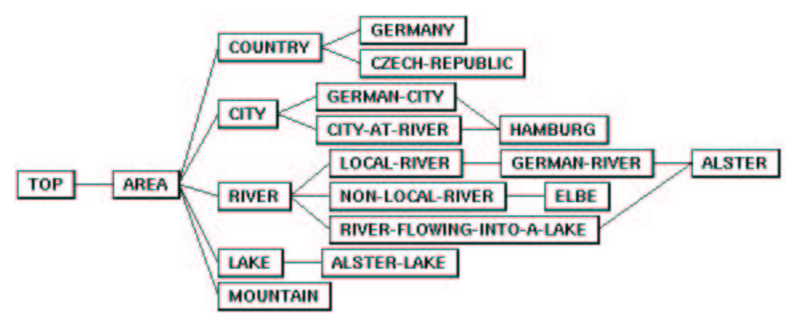
\includegraphics[width=0.85\columnwidth]{report7_figure6_taxonomy.png}
\caption{Computed taxonomy of the GIS example TBox from
  Wessel~\cite{Wessel2003}, Figure~6.
  The cover-tree tableau reproduces all 21 subsumption edges,
  including non-trivial spatial inferences such as
  Hamburg~$\sqsubseteq$~GermanCity (requiring RCC5 composition
  propagation through the PO-chain
  Hamburg--Alster--AlsterLake).}
\label{fig:gis-taxonomy}
\end{figure}

\begin{figure*}[ht]
\centering
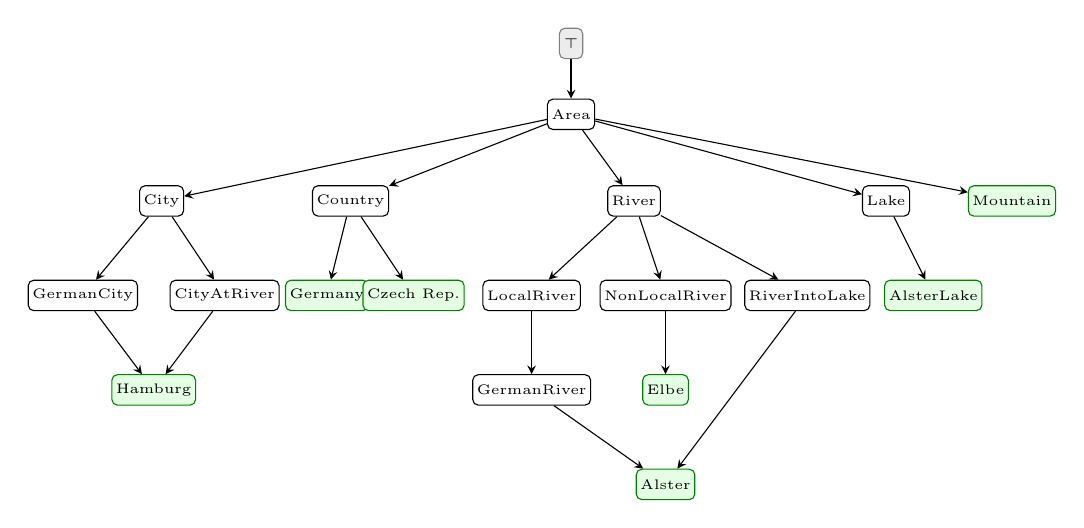
\begin{tikzpicture}[
  every node/.style={draw, rounded corners=2pt, font=\tiny,
    minimum height=1.1em, inner sep=1.5pt},
  leaf/.style={fill=green!10, draw=green!50!black},
  arr/.style={->, >=stealth, thin},
]
% Row 0: TOP
\node (top) [fill=gray!15, draw=gray] at (0,0) {$\top$};

% Row 1: Area
\node (area) at (0,-0.9) {Area};
\draw[arr] (top) -- (area);

% Row 2: Area's children
\node (city) at (-5.2,-2) {City};
\node (country) at (-2.8,-2) {Country};
\node (river) at (0.8,-2) {River};
\node (lake) at (4,-2) {Lake};
\node (mountain) [leaf] at (5.6,-2) {Mountain};
\draw[arr] (area) -- (city);
\draw[arr] (area) -- (country);
\draw[arr] (area) -- (river);
\draw[arr] (area) -- (lake);
\draw[arr] (area) -- (mountain);

% Row 3: children of City, Country, River, Lake
\node (germancity) at (-6.2,-3.2) {GermanCity};
\node (cityatriver) at (-4.4,-3.2) {CityAtRiver};
\node (germany) [leaf] at (-3.1,-3.2) {Germany};
\node (czech) [leaf] at (-2.0,-3.2) {Czech Rep.};
\node (localriver) at (-0.5,-3.2) {LocalRiver};
\node (nonlocal) at (1.2,-3.2) {NonLocalRiver};
\node (riverflowing) at (3.0,-3.2) {RiverIntoLake};
\node (alsterlake) [leaf] at (4.6,-3.2) {AlsterLake};
\draw[arr] (city) -- (germancity);
\draw[arr] (city) -- (cityatriver);
\draw[arr] (country) -- (germany);
\draw[arr] (country) -- (czech);
\draw[arr] (river) -- (localriver);
\draw[arr] (river) -- (nonlocal);
\draw[arr] (river) -- (riverflowing);
\draw[arr] (lake) -- (alsterlake);

% Row 4: deeper nodes
\node (hamburg) [leaf] at (-5.3,-4.4) {Hamburg};
\node (germanriver) at (-0.5,-4.4) {GermanRiver};
\node (elbe) [leaf] at (1.2,-4.4) {Elbe};
\draw[arr] (germancity) -- (hamburg);
\draw[arr] (cityatriver) -- (hamburg);
\draw[arr] (localriver) -- (germanriver);
\draw[arr] (nonlocal) -- (elbe);

% Row 5: Alster (two parents)
\node (alster) [leaf] at (1.2,-5.6) {Alster};
\draw[arr] (germanriver) -- (alster);
\draw[arr] (riverflowing) -- (alster);

\end{tikzpicture}
\caption{Taxonomy of the GIS example TBox, computed by the
  cover-tree tableau~\cite{GISTaxonomy}.
  Green nodes are leaf concepts (most specific).
  Note the DAG structure: \emph{Alster} has two parents
  (GermanRiver and RiverIntoLake) and \emph{Hamburg}
  has two parents (GermanCity and CityAtRiver).
  All 21~subsumption edges match Figure~\ref{fig:gis-taxonomy}.}
\label{fig:gis-computed}
\end{figure*}

%% ====================================================================
\section{History of Attempts (April--May 2026)}
\label{sec:history-of-attempts}
%% ====================================================================

The decidability argument summarised in
\S\ref{ssec:soundness-completeness} reached its current form
through seven rounds of adversarial review between Claude
(Anthropic) and GPT-5.5 (OpenAI) in April--May~2026, prompted by
Michael Wessel.  This section gives a compact abstracted
narrative of the evolution.  The full prose of each round, the
original superseded manuscripts, and the per-round repair list
are preserved in
\texttt{OUTDATED.md}~\cite{ALCIRCC5Outdated}.

\subsection{The starting point: cover-tree tableau + v1
completeness extraction (April 2026)}

The cover-tree tableau~\cite{CoverTree,CoverTreeImpl} and its
companion split-forest semantics~\cite{SiblingCompleted} were
established in April~2026 by GPT-5.4~Pro and
Claude~Opus~4.7, prompted by Wessel.  The split-forest paper
proves the soundness direction in full detail (Thms~1.17--1.19);
the converse---extracting a finite quotient from a satisfying
model---was given only as a proof sketch.  Claude wrote a first
attempt at the missing completeness extraction
(\textit{v1}~\cite{CompletenessExtractionV1}, April~2026).  In
parallel, the cover-tree implementation underwent two rounds of
adversarial review by Claude Opus~4.7 (April~17--18, 2026):
twelve implementation-level counterexamples were identified
across the $4\times 4$ grid of $(R_1,R_2)$ three-type chains
and the $\PP/\PPI$-transitive universal pattern, and all were
fixed in the shared \texttt{compute\_safe} helper and the new
Phase~5 / (CT5) role-path compatibility check
(Remark~\ref{rem:impl-bugs} above).  After these fixes the
911-concept cross-validation against the cycle-aware quasimodel
reasoner stabilized at $911/911$ matches with zero mismatches.

\subsection{v1 superseded, v2.1, and the round-2 31-page repaired
proof (May 6--12, 2026)}

GPT-5.5 reviewed v1 and identified two structural defects: the
Hasse construction for the cover-tree broke on infinite $\PP$-chains
(canonical example $C_\uparrow\equiv\exists\PP.\top\sqcap\forall
\PP.\exists\PP.\top$), and the $C5$ triple-coherence proof
conflated witnesses across pairs.  Claude responded with
\textit{v2}~\cite{CompletenessExtraction} (May~6) and
\textit{v2.1} (May~6).  A second-round review of v2.1 then
identified eight structural gaps, three load-bearing:
profile-port equality contradicted vertical separation on
self-loops via the $M1{+}M7$ reflexivity chain; the mate
construction forced all mates to share a single semantic parent
(refuted by the two-mate stress concept
$C_{AB}\equiv A\sqcap B\sqcap\exists\PP.A\sqcap\exists\PP.B\sqcap
\forall\PP.(A\to\lnot B)\sqcap\forall\PP.(B\to\lnot A)$); and
the rootless orientation was incompatible with the depth-from-$u_*$
projection.  GPT-5.5 produced a \textit{repaired
proof}~\cite{GPT55Repaired} (May~12, 16~pages) fixing all three
defects via occurrence-level equality, mates with different
parents, and request-closed cycles in place of
$\omega$-acceptance.  v2.1 was marked superseded; the repaired
proof was adopted as the current best statement.  Claude's
contribution shifted to verification:\@ six Python work packages
(WP1--WP6) cross-checking the repaired proof's finite
combinatorial content, all PASS.

\subsection{Rounds 3 and 4: structural layers added (May 13--21,
2026)}

Rounds 3 and 4 of GPT-5.5 review added four further structural
layers to the repaired proof, growing it from 16 to 31~pages:
(i) a verticalization discipline (mosaic axiom (M6)) stratifying
each context into a vertical stratum and a sibling frontier;
(ii) port-indexed mate clusters $\mathrm{Mate}_Q(C,s,p)$
attaching mate equivalences to contexts and ports rather than to
bare positions; (iii) an explicit abstract triple graph $T_Q$
with cardinality bounds; (iv) a side interface $\mathrm{Side}(u)$
with polynomial width bound $m(n)=O(n^3)$.  The certificate-space
bound $B(C_0)=2^{2^{p(n)}}$ became \emph{grammar-first}, derived
from these component bounds.

\subsection{Round 5: (M6$'$) recursive verticalization
(May 22--23, 2026)}

The round-5 review (GPT-5.5, May~22) identified a load-bearing
mathematical defect: the (M6) verticalization discipline was too
strong.  It forbade non-vertical $\PP/\PPI$ relations between
sibling-frontier mosaic positions, but such relations occur in
satisfiable witness-generated models---the round-5 stress
concept $\exists\DR.(A\sqcap\exists\PP.B)\sqcap\exists\DR.B$ is
SAT in abstract RCC5 yet rejected by (M6).  Eight repairs were
recommended.  Claude drafted two follow-up papers (the
(M6$'$) recursive-verticalization delta and the items-4-to-8
delta) that closed all eight items at the paper level, then
consolidated them into a 36-page round-5 v2 paper.  Side-witness
positions were allowed to open nested local vertical strata,
with the round-2 (M6) recovered as the depth-1 case.

\subsection{Round 6: internal-coherence pass (May 26, 2026)}

The round-6 review of the consolidated v2 (GPT-5.5, May~26)
found six internal-consistency gaps:\@ the old side-interface
lemma still asserted flat $\{\DR,\PO\}$ sibling frontiers; the
weakened per-position support closure (SC4$'$) was inconsistent
with the patchwork proof's per-triple appeal; overlap
universal-propagation was under-proved; the lasso construction
used the complete profile rather than the extended profile;
the side-width bound and validity-clause numbering were
inconsistent; and the verification script for the round-5
stress concept was not self-contained.  Claude drafted a
39-page round-6 internal-coherence pass closing all six gaps
and adding a self-contained pure-stdlib verification script
(\texttt{wp7\_selfcontained\_side\_witness.py}).

\subsection{Round 7: the abstract-position-symbol collapse
(May 27--28, 2026)}

The round-7 review of the round-6 paper (GPT-5.5, May~27)
identified one central architectural defect that could not be
locally patched.  Round-6 had defined the concrete pair label
by $\lab(u,v):=L_\Q(q(u),q(v))$, where $q:\Omega(\U(\Q))\to
\Pos_\Q$ sends each occurrence to an abstract position symbol
and $L_\Q$ is the abstract pair-label function with standard
reflexivity $L_\Q(\pi,\pi)=\EQ$.  In a finite regular
certificate the abstract position alphabet is finite while the
unfolding is infinite, so blocking deliberately reuses the same
symbol on fresh occurrences.  For the canonical one-state
upward cycle, distinct laps $u_i,u_j$ share the same symbol
$\pi$ and the round-6 rule gives $\lab(u_i,u_j)=L_\Q(\pi,\pi)
=\EQ$, even for $i\ne j$:\@ the strict $\PP$ chain collapses
into a $\PP$-self-loop.  The defect is intrinsic to indexing
labels by position-symbol pairs.

GPT-5.5's round-7 fix~\cite{GPT55Round7Sketch} replaces the
position-symbol pair labelling by labels on
\emph{occurrence-sensitive pair shapes} with explicit incidence
tags (described in~\S\ref{ssec:soundness-completeness}).
Twelve validity clauses (V1)--(V12) replace round-5 / round-6's
fifteen.  Claude wrote a round-7
audit/response~\cite{ClaudeRound7Audit} mapping the round-6
(G1)--(G6) and round-7 (D1)--(D5) defect lists to their
resolutions in the round-7 architecture, plus three further
self-contained verification scripts (WP7--WP9).  All of Claude's
round-5 / round-6 manuscripts are superseded by round 7 and
retained as the historical audit trail in
\texttt{papers/gpt5.5\_round2/}~\cite{ALCIRCC5Outdated}.

\subsection{Round 8: saturated side contexts and constructed
catalogues (May 28, 2026, evening)}

A fresh Claude~Opus~4.7 session, given the round-7 sketch with no
prior project context, identified three architectural defects.
First, the round-7 pair-shape enumeration did not exhaustively
cover the case of a side witness paired with a vertical-boundary
position:\@ a $\PP$ or $\PPI$ label between an exposed boundary
point and a side position could be hidden in the residual
$\DR/\PO$ frontier closure.  Second, the residual $\DR/\PO$
frontier restriction was imposed \emph{before} the side context
was saturated, making the restriction unsound while $\PP/\PPI$
pairs were still pending.  Third, the pair and triple catalogues
$\Pair_\Q$ and $\Tri_\Q$ were asserted finite but not explicitly
constructed.

GPT-5.5's round-8 repair~\cite{GPT55Round8Sketch} closes all
three by introducing a \emph{saturated side context} $S_k(u)$
generated by five (Sat1)--(Sat5) operations:\@ start with the
exposed vertical boundary of the source, add one selected witness
for each local $\exists R.D$ with $R\in\{\DR,\PO\}$ and modal
depth strictly less than $k$, recursively add smaller-depth
witnesses, assign or inherit a complete RCC5 label to every
ordered pair (including side/tree pairs), and close under
equality (label $\EQ$ triggers an equality-port declaration) and
containment (label $\PP$ or $\PPI$ triggers a local vertical
stratum) \emph{before} applying the residual $\DR/\PO$
restriction.  A new \emph{cross side/tree exhaustion lemma}
formalises that no $\PP/\PPI$ side/tree pair is hidden in the
residual frontier.  $\Pair_\Q$ and $\Tri_\Q$ are now constructed
as the least finite sets containing the explicit families of
pairs and triples generated by the saturated side contexts,
overlap amalgams, and residual configurations, with every triple
required to satisfy the RCC5 composition table.  The 15-page
round-8 sketch and the 30-page detailed
companion~\cite{GPT55Round8Expanded} are filed under
\texttt{papers/claude\_latest\_review\_gpt5.5\_fix/}.  Round-8 was
the most developed statement until a cold Opus~4.8 review found the
D-1 completeness gap (next); round-9 is its successor.

\subsection{Round 8 cold review: an open completeness gap (D-1) and
a proposed repair}
\label{ssec:round8-review}

A further cold review --- this time by Claude~Opus~4.8, again with
no prior project context --- examined whether the saturated-side-context
repair actually closes the side/tree gap, and found that it does
not:\@ it relocates the gap rather than closing it
\cite{Opus48Round8Review}.

The cross side/tree exhaustion lemma quantifies only over the
\emph{finite, depth-bounded} boundary $B_k(u)$ and the finite
saturated side context $S_k(u)$; both are bounded by the
side-width $m_\ast(C_0)$.  The lemma is true as stated, but the
advertised global conclusion --- ``no $\PP/\PPI$ side/tree pair is
hidden'' --- is a statement about the whole unfolded model, in
which the vertical ancestor chain is infinite.  The genuinely hard
case is a $\DR/\PO$ side witness that RCC5 composition forces to be
a proper part of an \emph{infinite} pumped tower.  The concrete
satisfiable witness is
\[
  G := (\forall\PO.X)\sqcap(\exists\PP.G),\qquad
  C_0' := (\exists\PP.G)\sqcap(\exists\PO.\neg X).
\]
$G$ generates an infinite ascending tower $a_1\PP a_2\PP\cdots$,
each $a_m\in\forall\PO.X$; the root's $\PO$-witness $w\in\neg X$ is
forced to satisfy $\rho(a_m,w)=\PPI$ for \emph{all} $m$ (base case:
$\rho(a_1,w)\in\comp(\PPI,\PO)=\{\PO,\PPI\}$, and $\forall\PO.X$ at
$a_1$ with $w\in\neg X$ kills the $\PO$ option; induction:
$\comp(\PPI,\PPI)=\{\PPI\}$).  Only finitely many tower nodes fit
in $S_k(u)$; for the unbounded tail the constructed pair-shape
catalogue offers no admissible shape ($\side_{\PPI}$ needs
co-residence in one bounded context; $\down$ needs a cover-edge
path the construction never creates for a side witness;
$\front_{\DR}$ is composition-illegal; $\front_{\PO}$ violates the
$\forall\PO.X$ universal-safety check).  So the round-8 completeness
construction produces an invalid certificate for the satisfiable
$C_0'$ --- a genuine gap (``D-1''), of medium--high severity.  The
composition arithmetic is machine-checked.

The decidability \emph{theorem} most likely survives:\@ placing
$w$ as a true vertical descendant of the tower (a selected
$\Eup$-child of $a_1$, with the $u$--$w$ edge demoted to a residual
$\PO$ frontier) appears to yield a valid certificate, and the
decision procedure accepts whenever \emph{some} valid certificate
exists.  The accompanying repair note~\cite{Opus48Round8Repair}
turns this observation into a construction --- \emph{composition-forced
verticalization}: detect when composition forces a $\DR/\PO$
witness to be a proper part of an ancestor, and splice an $\Eup$
cover edge at the (provably bounded) threshold height where it
first becomes a proper part, so equality-aware reachability carries
the correct $\PP/\PPI$ label up the entire tail.  Three facts make
the repair clean, the first machine-checked:\@ (i) the forced label
up an ascending chain is monotone in $\DR\succ\PO\succ\PPI$ and
$\PPI$-absorbing, hence eventually constant at a threshold; (ii)
the threshold is bounded by the number of boundary descriptors, so
finiteness is preserved; (iii) the construction \emph{presents a
fixed consistent model}, so RCC5 composition and universal safety
are inherited rather than re-derived.  The cold reviewer recorded
this as a candidate with open bookkeeping obligations; GPT-5.5 then
took it up in round-9 (next).

\subsection{Round 9: composition-forced verticalization closes D-1
(May 29, 2026)}
\label{ssec:round9}

GPT-5.5 ratified the D-1 defect and integrated the cold reviewer's
repair into a round-9 proof~\cite{GPT55Round9Sketch} (16-page
sketch) with detailed companion~\cite{GPT55Round9Expanded}
(33~pages), filed under \texttt{papers/gpt5.5\_round3/}.  A 5-page
formal response memo~\cite{GPT55Round9Response} records that GPT-5.5
re-ran the three Opus~4.8 verification scripts (all pass), confirmed
the composition facts $\comp(\PPI,\PO)=\{\PO,\PPI\}$ and
$\comp(\PPI,\PPI)=\{\PPI\}$ that drive the phenomenon, and agreed
that ``this is a genuine completeness defect, not merely a
presentational ambiguity.''

Round-9 distinguishes two cases for a selected $\DR/\PO$ side
witness $w$ of a source $u$.  If its relation to the ancestor tower
remains $\DR/\PO$, $w$ stays an ordinary side witness and deep
ancestor--witness pairs are residual $\DR/\PO$ pairs.  If RCC5
composition forces $w$ to be a proper part of all sufficiently high
tower nodes, the proof inserts a generated cover edge
$w'\,\Eup\,a^\ast$, where $a^\ast$ is the first retained
representative of the eventual $\PPI$-tail and $w'$ is $w$ or a
split equality mate; every later pair $(a_m,w')$ is then presented
by equality-aware vertical reachability.  This is a presentation
change, not a semantic change:\@ the splice is added only when the
inherited satisfying model already has $w'\PP a^\ast$, and the
$u$--$w$ relation stays the inherited $\DR/\PO$ residual pair.

Three lemmas carry the repair.  \emph{Monotone ancestor traces}:\@
for a $\DR/\PO$ witness $w$ of $u$ and a tower $u<a_1<a_2<\cdots$,
the trace $r_m=L(a_m,w)$ has shape $\DR^*\PO^*\PPI^*$ ($\EQ,\PP$
impossible; $\PPI$ absorbing because $\comp(\PPI,\cdot)$ never
increases rank).  \emph{Bounded threshold after regular
replacement}:\@ augmenting the tower descriptor with the
three-valued trace status leaves finitely many descriptors, so each
of the at most three constant regimes needs only boundedly many
representatives and the first retained $\PPI$-point sits at a
computable height $N_{\mathrm{thr}}(C_0)$.  \emph{Global residual
frontier}:\@ after equality ports, finite containment saturation,
and forced verticalization, every remaining residual-frontier pair
has label $\DR$ or $\PO$.  The split-cover and extraction proofs are
updated to apply the forced-verticalization test before ordinary
side-context attachment.

The repair preserves the no-automata split-forest architecture (no
B\"uchi/parity automata); the only extra finite information is the
three-valued ancestor-trace status, absorbed into the existing
finite-index replacement argument.  On the computational side, the
round-9 construction is exercised end-to-end by a certificate-emission
test on $C_0'$ and its UNSAT sibling, generalised to a parameterised
forced-tower family and cross-checked against a by-construction oracle
and the cover-tree tableau (\S\ref{ssec:compverif}); this closes the
round-8 review's recommendation to add $C_0'$ as a constructive
emission test.  GPT-5.5 explicitly characterises
round-9 as ``a serious proof manuscript rather than a mechanically
certified theorem,'' naming the bounded-threshold replacement lemma,
the typed-equality quotient lemma, and the support-closed mosaic
patchwork theorem as the parts most worth future formalization.
When written, round-9 was \emph{strongly supported but not
certified} and the most developed statement of the no-automata thread.
It was then cold-reviewed in turn---which found a dual descendant-tower
defect and two foundational gaps---and superseded within the day, as
the next subsection records.

\subsection{Round 9 cold review, round 10, and the switch to the
automata route (May 29, 2026)}
\label{ssec:round10-automata}

A fresh GPT-5.5 session, given the round-9 manuscripts with no project
context, reviewed round-9 and found it was not yet a proof.  The
composition table was independently re-verified correct.  Three
\emph{critical} defects:
\begin{itemize}
  \item \textbf{One-sided verticalization.}  Round-9 handled a
    $\DR/\PO$ witness forced into an infinite \emph{ancestor}
    $\PPI$-tower but missed the dual case --- a $\PO$ witness forced
    to be a proper \emph{superpart} of an infinite \emph{descendant}
    $\PP$-tower.  Concrete witness
    $C=(\exists\PO.A)\sqcap(\exists\PPI.\top)\sqcap
    \forall\PPI.(\exists\PPI.\top\sqcap\forall\DR.\neg A\sqcap\forall\PO.\neg A)$:
    each descendant $d_i$ is forced
    ($\comp(\PP,\PO)=\{\DR,\PO,\PP\}$, $\DR/\PO$ killed by the
    universals, $\comp(\PP,\PP)=\{\PP\}$ absorbing) to satisfy
    $d_i\PP w$ (machine-checked).
  \item \textbf{Finite checkability never proved.}  The validity
    clauses (V6)/(V7) were \emph{asserted} to be finite syntactic
    checks but quantify over the infinite unfolding; the finite
    pair/triple catalogues were never shown to exhaust it.
  \item \textbf{Boundary non-determinacy.}  A boundary descriptor
    does not determine the mixed outside/internal labels:\@
    $i\PP b,\ o\PO b\Rightarrow L(o,i)\in\{\DR,\PO,\PPI\}$.
\end{itemize}
plus four majors, including a \emph{false} simple-cycle bound (a
request-closed cycle may need a closed walk that revisits
descriptors).

Round~10 accepts all findings and repairs them:\@ a dual descendant
splice (symmetric to round~9), occurrence-local requests, ranked
side-width, global-quotient-before-cycle-selection, a corrected
$(M{+}1)N$ closed-walk bound, and --- for the two foundational
criticals --- a \emph{finite product-state exhaustion} construction
and \emph{complete interface descriptors}.  A close reading finds
that the entire decidability burden then funnels into two named
lemmas, Finite Product Exhaustion and Complete-Interface Replacement,
both established by case analysis plus finiteness of a descriptor
alphabet, and both \emph{automaton-shaped}: product-state exhaustion
is product-automaton reachability, and the complete interface
descriptor is a finite interface abstraction.

This is the convergence point.  Over rounds 2--10 the no-automata
route repeatedly rediscovered automaton-shaped obligations
(request-closed cycles for $\omega$-acceptance; product-state
exhaustion for finite checking) that it could not discharge.  The
decision (29~May~2026) is therefore to promote the split-forest
$+$ parity-tree-automata proof~\cite{GPT55AutomataRoute}
(\S\ref{ssec:soundness-completeness}) to the primary statement: it
keeps the entire split-forest normal form and lets a parity tree
automaton --- whose non-emptiness is decidable by construction ---
handle the brittle half directly.  The promotion was strategic, not a
proof upgrade; the automata proof was then cold-reviewed in turn (the
5th cold review), found to share the finite-representation keystone gap,
and repaired; its finite-abstraction keystone (Theorem~B) was then
cold-reviewed in turn (the 6th cold review) and found unproved,
prompting GPT-5.5's round-12 patchwork-bag repair (global RCC5
consistency via the patchwork property, decided by a two-way parity
automaton), which is now the canonical statement and has not itself
been cold-reviewed.

\subsection{What survives, and why}

The split-forest architecture itself---witness thinning,
generated containment covers, weak-EQ split copies for multiple
selected $\PP$-superparts, sibling interfaces recorded by
finite support-closed mosaics with $\{\DR,\PO\}$-only open
cross-relations, typed equality-port congruence quotient to
recover strong-$\EQ$ semantics, and request-closed cycles---is
present in every round from v1 through round~7.  What changed
was \emph{how labels are indexed on this architecture}.  The
v1, v2, v2.1, and round-2 versions indexed labels by the rank-$d$
quotient and abstract position symbols; the round-7 architecture
indexes them by occurrence-sensitive pair shapes.  The whiteboard
sketch (Wessel), the DR-rigidity insight, the EQ-splitting and
typed-EQ-quotient idea, the cover-tree decomposition, GPT-5.4's
v1 formalisation, and Claude's cover-tree tableau implementation
all remain load-bearing in round~7.

\subsection{Computational verification across rounds}
\label{ssec:compverif}

In parallel with the proof work, nine Python work packages
verify the finite combinatorial content of the proof family.
WP1--WP6 verify the round-2 31-page repaired
proof~\cite{GPT55Repaired} and all PASS:\@ brute-force
enumeration confirms the RCC5 composition table in all 25
cells (WP1); a validity-condition checker accepts $C_\uparrow$
via parent self-loops, accepts $C_{AB}$ via two mates with
different parents, and rejects the v2.1-style single-parent
$C_{AB}$ attempt (WP2); a small-model SAT/UNSAT oracle exhibits
a concrete 3-element model for $C_{AB}$ (WP3); $C_{AB}$ and
request-closed cycle tests fold into WP2/WP3 (WP4, WP5); a
mosaic enumeration confirms support-closure axioms on small
mosaics (WP6).  WP7--WP9 verify the round-7 central stress
concepts (comparable side witnesses, blocking-not-equality, and
split copies for incomparable proper superparts).  WP10 drives the
D-1 witness $C_0'$ end-to-end through the round-9 forced-verticalization
construction---detect the forced ancestor trace, splice at the bounded
threshold, build the incidence-tagged certificate, validate the round-9
clauses---emitting a valid certificate for $C_0'$ and rejecting its
UNSAT sibling; WP11 generalises this to a parameterised forced-tower
family (period-$p$ profiles, many side witnesses, universals over
$\{\PO,\PPI,\DR,\PP\}$) and cross-checks the round-9 emit/reject verdict
against a by-construction oracle, an independent certificate validator,
and the cover-tree tableau ($216/216$ agreement on the current sweep,
no completeness or soundness gap found on that family; the
overlap-amalgam case remains future work).  WP10/WP11 close the
round-8 review's recommendation to add $C_0'$ as a constructive
certificate-emission test.  All PASS.  No counterexample to any
combinatorial claim of any round was found.

%% ====================================================================
\section{Outlook and Conclusion}
\label{sec:outlook}
%% ====================================================================

\subsection{Preliminary conclusion (end of May~2026)}
\label{ssec:prelim-conclusion}

We state the status plainly, as it is provisional.  The decidability of
$\ALCIRCC{5}$ \emph{remains open} (and $\ALCIRCC{8}$ likewise); as of the end of
May~2026 the decidability argument is \emph{strongly supported but not
certified}.  Two layers should be kept apart.

\emph{The settled foundation} is the split-forest model class---the semantic
normal form of Theorem~A (witness thinning, generated containment covers, split
copies for incomparable superparts, side-interface mosaics, typed-$\EQ$
quotient).  Every satisfiable concept admits a witness-generated, tree-like
split-forest model, and this normal form has been found sound by \emph{every one
of the six cold reviews} conducted on the project---it is the one component that
has never broken.  Everything downstream is built \emph{on top of} it: the finite
patchwork-bag abstraction and the two-way alternating parity tree automaton
\emph{consume} the split forest rather than replace it.

\emph{The open layer} is exactly that finite abstraction.  The current canonical
manuscript (round~12) replaces the earlier transformer-based abstraction---which
a cold review found unproved---by a patchwork-bag abstraction whose global RCC5
coherence follows from the patchwork property of RCC5, with infinite
eventualities decided by two-way parity-automaton emptiness.  It is a complete,
self-contained manuscript that \emph{proves} its finite-abstraction adequacy on
paper, modulo two standard external theorems (the RCC5 patchwork property;
emptiness of two-way alternating parity tree automata).  A subsequent
self-contained 29-page edition makes this fully explicit, expanding the
theorem spine with appendices that discharge every load-bearing step---in
particular deriving the global RCC5 labelling by a compactness argument over the
finite relation alphabet (given finite patchwork), with no route-dependent
transformer, which is precisely the global-coherence step the cold review had
faulted in the earlier transformer-based abstraction.  What the manuscript has
\emph{not} yet received is an independent cold review or a machine-checked
certification.
``Strongly supported, not certified'' should be read in precisely this
sense---proved on paper, not independently verified---and not as a claim that any
step is known to be missing.  \emph{(Update, July~2026: that last clause has
since been overtaken---the seventh review identified one concretely unproved
step; see \S\ref{ssec:july2026-update}.)}

The trajectory across the rounds is convergent: the repairs have moved from
bespoke, hand-built machinery towards standard, citable theorems, so we regard
the present state as a natural consolidation point.  Settling the question
definitively will require either mechanization (Lean/Coq) of the
finite-abstraction keystone---axiomatizing the two external theorems and
formalizing the normal form and the adequacy argument---or human expert peer
review.  Until then we offer the work as a discussion piece: a problem open for
over twenty years, with the standard undecidability routes shown blocked and a
convergent-but-uncertified decidability argument resting on the sound
split-forest model class.


\subsection{Update (July 2026): the seventh review}
\label{ssec:july2026-update}

The consolidation stance above held for five weeks, until a genuinely stronger
reviewer became available: Claude Fable~5 (Anthropic's first Mythos-class
model, a capability tier above Opus, and a different model lineage from the
round-12 author, GPT-5.5).  A materially stronger reviewer is itself new
information, so the freeze was broken once for a \emph{seventh review}---a
context-loaded (``hot'') adversarial audit of the canonical round-12
manuscript, explicitly \emph{not} a cold review, accompanied by three new
computational work packages (WP14--WP16); see
\texttt{papers/fable5\_review/} in the repository for the full report and
probes.  It continued the series' pattern: every review so far has found a
defect, and this one did too (seven reviews, seven defects).

The critical finding is that the round-12 truth lemma rests on an unproved
\emph{shadow-amalgamation} step: the global RCC5 relation $\rho_T$ is
amalgamated by patchwork from the \emph{bag networks only}, yet the lemma
assumes the declared relation-vector shadow entries agree with $\rho_T$.  No
legality test constrains two shadows against each other, and the implicit
lemma---bags plus all declared shadow rows are jointly realizable in one
frame---is in fact false for the tests as written: WP15 exhibits a three-bag
configuration (declared entries $x_1\,\DR\,x_2$, $x_1\,\PP\,p$,
$x_2\,\PPI\,p$; $\comp(\PP,\PP)=\{\PP\}$ forces $x_1\,\PP\,x_2$) that passes
every listed test and admits no realizing frame; 23 of 64 assignments on the
minimal pattern fail.  This is the sixth review's transformer-coherence gap
recurring one layer up, but strictly smaller: the single-shadow case is
provable from the patchwork theorem itself, and no counterexample exists
under a \emph{vertical-liveness} repair discipline ($\PP/\PPI/\EQ$ pairs
always co-bagged, shadow entries restricted to $\{\DR,\PO\}$---the
saturation rules extended to the shadow layer; 358/358 random and exhaustive
configurations clean) or under an extended-bag discipline (200/200).  Two
specification loopholes were also found ($\EQ$-valued shadow entries;
undefined shadow propagation scope), each independently soundness-fatal as
literally written and each a one-line fix: WP16 machine-checks that either
loophole makes the mechanism wrongly accept four unsatisfiable
forced-composition concepts, while under the repaired discipline it agrees
with the cover-tree tableau on all ten referee diagnostics---including,
notably, the strong-$\EQ$ PO-loop concept that the retired quasimodel
reasoner decided wrongly---and on a 148-concept random sweep without
disagreement.  The $K(C_0)$ finiteness argument also remains an assertion.

What held up under attack is equally important: the RCC5 patchwork theorem
\emph{in exactly the round-12 form} was verified exhaustively at small
widths (WP14: 63{,}219 two-bag amalgamations and 300 tree-of-bags patchings
executed literally along the manuscript's own induction, zero failures), as
did the finite-to-countable compactness passage, strong equality, the
running-intersection layer, and Theorem~A's normal form.  No
accepted-but-unsatisfiable \emph{concept} was found.  The status label is
therefore unchanged---\emph{strongly supported, not certified}---with the
keystone sharpened from ``patchwork-bag adequacy'' generically to a
\emph{shadow-amalgamation lemma} (plus the $K(C_0)$ accounting)
specifically.  The consolidation stance otherwise stands: mechanization or
human peer review remain the decisive next steps, with frontier-model audits
as the sanctioned exception whenever a genuinely stronger reviewer appears.


\paragraph{Round 13 (July 2026, unreviewed).}
The seventh reviewer then executed its own repair programme
(\texttt{papers/fable5\_round13/} in the repository): a ten-page delta on
round-12 that tightens the abstraction language --- shadow entries
restricted to the horizontal relations $\{\DR,\PO\}$, with vertical and
equality relationships co-bagged (the existing saturation and
residual-frontier regime extended to the shadow layer), mandatory shadow
propagation with a verticalization fallback, type-propagation of
transitive vertical universals, request-source liveness, and a
pair-coherence rule --- and, under that discipline, \emph{proves} the
previously missing shadow-amalgamation lemma from four exhaustively
machine-checked composition-table facts plus the patchwork-and-compactness
apparatus; the truth lemma then holds with the declared shadow entries
literally equal to the amalgamated relation.  The residual proof burden
moves, explicitly, to the completeness side (a coverage lemma, and the
interaction of on-demand verticalization with the effective width bound),
which the manuscript designates as the next review target; the effective
width bound itself is re-derived from a witness-generated accounting.  A
further harness (WP17) checks the finite facts exhaustively and the
lemma's constructive content on four hundred random tree-shaped
configurations, with a functioning negative control.  Round 13 is
authored by the reviewer, is unreviewed, and inherits the project's
presumption of a defect until a genuinely cold review fails to find one;
the status label is unchanged: strongly supported, not certified.


\paragraph{Round 14 (July 2026, GPT-5.5; the eighth review).}
The presumption was correct.  Handed a targeted task packet for round 13's
self-designated weak points, GPT-5.5 broke the round-13 extraction clause
exactly there (the eighth review; eight reviews, eight defects): the
satisfiable tower concept
$\exists\PP.\top\sqcap\forall\PP.(\exists\PP.\top\sqcap(\forall\PP.\exists\PP.\top
\sqcap\forall\DR.A))$ gives every tower level a horizontal universal
obligation, and round 13's literal propagation-with-verticalization clause
then forces every remote level into the root bag --- unbounded width for a
fixed concept, machine-checked; a second finding shows mixed
$\PP/\PPI$ paths defeat the orientation assumption of the type-propagation
rule.  The shadow-amalgamation lemma itself survived re-testing.  GPT-5.5's
round-14 repair withdraws the horizontal-shadow discipline in favour of the
\emph{active-virtual-bag} form of the extended-bag route (the alternative
the seventh review had outlined): every universal source is treated as a
virtual active occurrence at every bag, with exact --- possibly vertical ---
relation vectors; validity requires every \emph{finite} restriction of an
active bag to be a closed complete atomic RCC5 network, with adjacent
agreement; patchwork and compactness then realize all declared values
verbatim, the coverage lemma becomes trivial, and extraction adds no live
ports (the tower is absorbed with two live ports and virtual shadows).
Claude reproduced all seven new harnesses and hot-audited the manuscript;
the designated cold-review targets are the automaton's pair/triple monitor
bookkeeping (self-flagged by the author), the explicitness of the
single-shadow closure check, and the inherited width accounting.  Two
structural observations deserve record: both the seventh and eighth defects
were found precisely where the preceding round's ``what would invalidate''
list pointed, and the two model lineages have now each broken and each
repaired the other's round --- the review-and-designate discipline is
functioning as designed.  Status unchanged: strongly supported, not
certified; a genuinely cold review of round 14 is the next step.


\paragraph{The ninth review (July 2026, cold): the decision layer is the gap.}
Round 14 was then reviewed \emph{cold} by a fresh session of the strongest
available model, per the project's packet protocol (manuscripts only; all
prior reports withheld).  The verdict was \emph{gap}, with the most precise
delimitation the project has had.  On the positive side, the reviewer
\emph{reconstructed} --- not merely read --- the active-virtual-bag semantic
layer and found it sound, calling its amalgamation and truth lemmas the
strongest versions of these results in the stack's history; strong equality
survived its sharpest uniqueness probes in both directions; the composition
table and the small-width patchwork instances were re-derived from scratch.
On the negative side, the critical finding is structural: a valid
active-virtual-bag abstraction is a \emph{pair} --- a finitely-labelled tree
plus an unbounded relational enrichment that is not carried by any label ---
so the automaton theorem must decide an existential-\emph{projection}
language, a statement the stack never formulates; and the sketched monitor
design is \emph{unsound as described}, because independent alternating run
copies cannot be forced to guess the off-label data consistently (the
reviewer exhibits a machine-checked configuration in which every sketched
check passes while no coherent enrichment exists, the required value being
pinned to the empty set $\comp(\PP,\PP)\cap\comp(\PP,\DR)=\varnothing$).
Three natural repairs (label annotation, profile quotienting, canonical
guessing) are each shown blocked by facts the stack itself establishes.
Two further findings concern the width layer: the liveness cost of deferred
existential requests is never integrated into the width accounting, and the
surviving width lemma's recurrence does not close as written (its witness
generation can cascade at fixed rank; the identified fix is a single
decreasing measure).  The reviewer's structural summary deserves quotation:
across the last three rounds ``the gap has migrated; it has not closed'' ---
from bounded labels with an unproved existence claim, to restricted rows
that broke width, to total semantic data with no decision procedure.  The
ledger stands at nine reviews, nine defects; for the third time, a cold
review found what context-loaded audits had missed.  The recommended
round-15 alternatives are a bounded-interface or uniformization lemma making
the enrichment label-representable, or abandoning the tree-automaton layer
for a mosaic/type-elimination decision procedure running directly on the
infinitary abstraction, whose model-construction half the review certifies
as already in place.  Status unchanged: \emph{strongly supported, not
certified} --- a semantic theory in the best shape it has ever been, and a
decision layer that remains unwritten.


\paragraph{Round 15 (July 2026): the decision layer, without automata.}
Executing the ninth review's second alternative, round 15 removes the
automaton layer entirely and replaces it by a \emph{cluster quasimodel}
certificate: a finite set of Hintikka types with safe links, a finite
catalogue of small closed atomic cluster patterns in which every
existential demand is fulfilled within one gluing step (so there are no
promissory witnesses and no parity condition at all --- the deferral
defects of the early rounds are structurally excluded), long-range
conditions over a newly isolated \emph{fold lattice} --- the closure of
the RCC5 atoms under set-composition, shown by exhaustive machine check
to contain exactly ten sets, each a vertical singleton or containing a
horizontal atom --- and a shared core cluster for uniquely realizable
types (absorbing the ninth review's shared-witness probe with no
liveness cost).  Global coherence is constructed once, in the soundness
proof, by iterated patchwork over the unfolding together with a
canonical horizontal selection on the fold lattice; no run-time device
guesses anything, so the ninth review's critical finding does not apply
structurally.  The width bound is re-proved under a single strictly
decreasing measure, resolving the review's third finding, and the sole
remaining external input is the RCC5 patchwork property --- the two-way
parity-automaton emptiness dependency is gone, which also shortens the
eventual mechanization path.  A new harness checks the fold lattice
exhaustively, probes the steering keystone on 250 random glue steps
(all realizable; a negative control fails as it must), and
cross-validates the acceptance semantics against the cover-tree tableau
on all eleven historical diagnostics plus a 200-concept random sweep
with no disagreements.  Round 15 designates its own weak points (the
steering induction, the horizontal normal form for extraction, and
one-step saturation at bounded width), is authored by the same lineage
that wrote round 13, and is unreviewed: after nine reviews and nine
defects it should be presumed to contain the tenth until an adversarial
review --- next, by the other lineage --- fails to find it.  Status
unchanged: \emph{strongly supported, not certified}.


\paragraph{What survives of the split-forest models in round 15.}
Since the decision layer has now changed shape three times, it is worth
stating precisely how much of the original split-forest model class
(GPT-5.4, April 2026) is still load-bearing.  The answer is: essentially
all of the model theory, and none of the successive decision machinery.
Witness thinning is unchanged and remains the first step of the
extraction.  The saturated side contexts survive \emph{verbatim} --- the
round-15 cluster patterns are exactly the saturated bags of Theorem A,
and the one-step demand condition is the saturation discipline restated.
Split copies for incomparable superparts survive as the gluing
interfaces of the pattern catalogue (running intersection playing the
role of the old overlap maps).  The generated containment forest
survives as the \emph{unfolding}: infinite towers are infinite chains of
pattern copies, and the old vertical-closure lemma
($\comp(\PP,\PP)=\{\PP\}$) survives as the transitive-safety condition
together with the singleton case of the fold analysis.  Strong equality
as exact occurrence identity survives and is extended by the core
cluster, which gives semantically unique elements one global occurrence
rather than quotienting copies.  Finally, the residual-frontier
principle of the early rounds --- only $\DR/\PO$ may remain
unrepresented --- reappears, generalized and machine-checked, as the
fold-lattice fact that every unrepresented long-range relation is
chain-forced vertical or admits a horizontal value.  What has been
discarded along the way is exactly the succession of decision devices:
the hand-written certificate clauses of rounds 2--10, the interface
transformers of round 11, the relation-vector shadows of rounds 12--13,
the guessed enrichment and parity automata of rounds 11--14.  In this
sense the round-15 certificate is the most literal finite image of the
split-forest model class the project has produced: it \emph{is} the
split forest, folded by pattern isomorphism, with the fold lattice
bounding what the folding forgets.


\paragraph{The tenth review (July 2026): round 15 falls at its designated
keystone.}
GPT-5.5's targeted pass broke round 15 exactly where the manuscript
pointed: the steering condition of the canonical completion is stated
pairwise (each unrepresented pair must admit a safe horizontal value in
its fold), and a minimal machine-checked witness --- two safe sets
$\{\PO\}$ and $\{\DR\}$ over an already-realized $\PP$ edge, with
$\comp(\PP,\DR)=\{\DR\}$ pinning the pair the first set cannot reach ---
shows the pairwise condition passes while no joint completion exists.
The post-mortem sharpened the finding: the witness configuration is
semantically unrealizable, so the condition accepts what it should
reject, and the repair --- making the condition \emph{joint}, requiring
a closed completion of the finite domain problem per gluing profile ---
provably cannot hurt completeness, since extraction from a real model
always supplies the joint solution.  The review also exposed a
spec-versus-test mismatch in the accompanying harness, which had
validated a stronger discipline than the manuscript stated; the harness
now tests the condition as written and confirms the defect at scale.
The ledger stands at ten reviews, ten defects, and the failure genus is
the project's single recurring shape --- pointwise checks that do not
compose jointly --- in its fourth incarnation.  Two things did not
break, again: the split-forest model class, and the round-15
architecture around the failed condition (the fold lattice, one-step
clusters, and the core were not reached).  The round-16 direction is
fixed and small: replace the pairwise steering condition by the joint
per-profile amalgamation check.  Status unchanged: \emph{strongly
supported, not certified}.


\paragraph{Round 16 (July 2026): the joint selection becomes certificate
data.}
The repair of the tenth defect implements the reviewer's own closing
recommendation: the certificate now stores, per gluing edge, a
\emph{steering function} from finite interface states (type, row over
the separator, safety signature) to fresh rows, subject to four finite
conditions including a pair condition over the \emph{reachable} pair
states --- computable from the certificate itself by a least fixed
point, because every long-range value in the unfolding is generated by
the certified functions.  The canonical completion of the soundness
proof thereby becomes deterministic: no pointwise choice survives
anywhere, each triangle class is discharged by a certified condition,
and the tenth review's witness family is provably rejected (machine
checks: soundness on all accepted random glue steps, zero false
accepts).  The residual debt is concentrated in one named and
\emph{measured} obligation: the uniformization lemma --- extraction
must factor the model's per-instance values through states --- which at
the coarsest granularity fails on $1.4\%$ of random jointly-realizable
steps, with two finite repair routes identified; soundness does not
depend on it, so the risk direction is over-rejection only.  The ledger
stands at ten reviews, ten defects; round 16 is reviewer-authored and
unreviewed, and should be presumed to contain the eleventh.  Status
unchanged: \emph{strongly supported, not certified}.


\paragraph{The eleventh review (July 2026, cold): the first no-counterexample
verdict.}
The round-16 stack was cold-reviewed by a fresh session of the other
lineage.  For the first time in eleven reviews, the referee found
\emph{no counterexample and no false lemma}: the verdict is ``gap ---
not certified as written,'' with the explicit assessments that no
algebraic counterexample to the intended theorem was found, that the
four-class triangle taxonomy is algebraically adequate under
strengthened invariants, that the uniformization delimitation is sound
(failure would mean over-rejection, not wrong answers), and that with
six named repairs ``the intended soundness argument [is] very likely
correct.''  The repairs demanded are formalization obligations rather
than corrections: an explicit finite transition system for the
reachability fixed point, an ordered-pair transport rule (supplied
verbatim by the reviewer), a proved operational-inclusion invariant
including the shared-core case, the separator-covers-core statement,
explicit pair orientation, and stored witness choices; the width
budgets remain the standing deeper item, alongside uniformization.  The
reviewer independently re-derived the ten-set fold lattice, matching
the project's computation exactly.  The ledger is now eleven reviews:
ten defects with witnesses, and one demand for unwritten formalization
--- the qualitative shift the choice-free round-16 design was built to
force.  The status label does not change on one such verdict:
\emph{strongly supported, not certified}.


\paragraph{Round 17 (July 2026): the work order implemented.}
Round 17 supplies everything the eleventh review demanded: the gluing
normal form (every pre-existing member of a new pattern copy lies in
the separator; separators consist of parent-copy members and core
references; the core is a permanent interface at every step), the
explicit finite transition system (singleton states with persistent
core rows and a total three-case row decomposition; ordered pair states
with simultaneous converses, seeded, created at birth, and transported
by the reviewer's own rule, underpinned by a no-overwrite lemma), a
\emph{proof} of the operational-inclusion invariant --- every state and
every ordered pair actually occurring in an unfolding lies in the
computed reachable sets, with the shared-core cases discharged by core
persistence and birth-pattern membership --- and a stored witness map
making the canonical unfolding a function of the certificate, so the
determinism claim is exact.  An executable rendering of the system
verifies the inclusion invariant on twelve hundred random unfoldings
without a violation and confirms that the transport rule is
load-bearing (birth-only fixed points miss transported pairs in every
catalogue that has them).  By the eleventh reviewer's stated criterion,
the soundness half of the decision layer is now fully written ---
explicit system, proved inclusion, no free choices --- and, being
literally in transition-system form, has become a transcription target
for mechanization rather than a research problem.  The delta is
unreviewed; the completeness side retains its two named open lemmas
(the width budgets and uniformization).  Status unchanged:
\emph{strongly supported, not certified}.


\paragraph{The twelfth review (July 2026): the transport rule has a seam.}
Framed as an acceptance test against the eleventh review's own work
order, the twelfth review rejected round 17 on a precise, finite
finding: the written ordered-pair transport rule fires only when both
endpoints are updated by the ambient transition, while a pre-existing
member of the parent copy outside the child separator receives a
birth-adjacent catalogue state instead --- so mixed ambient/parent-copy
pairs silently escape the fixed point, the pair condition never
inspects them, and the round-16 counterexample triangle recurs at
exactly that seam (machine-checked, reproduced).  Two instructive
meta-findings accompany it: the executable harness had implicitly
implemented the correct \emph{total} transport, which is why twelve
hundred simulations showed nothing --- the defect lives in the written
rule, not the intended construction --- and the harness itself was
caught being hash-seed-nondeterministic.  The stack also grew stronger
where it held: the reviewer failed to break the parent-plus-core normal
form and volunteered the running-intersection argument for its
extractability, found no overwrite witness, and discharged the
ordered-pair item cleanly.  The ledger stands at twelve reviews: eleven
defects with witnesses, one no-counterexample verdict.  The round-18
repair is fully specified by the reviewer (a total endpoint-update
operation, transport under it, the re-proved inclusion case analysis,
defined path semantics, and a deterministic branching harness).
Status unchanged: \emph{strongly supported, not certified}.


\paragraph{Round 18 (July 2026): total transport, and the birth flip.}
Round 18 implements the twelfth review's repair package in full, with
one sharpening that working out the demanded path semantics forces: the
total endpoint update has \emph{three} clauses, not two.  Besides the
review's ambient case (recorded steering rows carried forward) and
resident case (catalogue read-off), cross-branch occurrences require a
\emph{birth-flip} clause --- a younger occurrence's entry to an older
separator member is the converse of the steering value the older side
received at the younger's birth --- which is precisely the
least-common-ancestor role change the review had flagged as undefined.
A birth-dichotomy lemma (at every step, every pre-existing occurrence
is co-patterned or steered; there is no third case) makes the update
total and every pair value single-assignment; pairs are transported in
lockstep; the inclusion theorem is re-proved by a five-way
endpoint-class analysis in which the review's mixed seam becomes an
ordinary transport step; and an order-invariance lemma derives the
path semantics.  The accompanying harness makes the review's
methodological lesson structural: states are computed from the written
rules alone, never from the realized structure, and cross-checked
against ground truth on genuinely branching unfoldings --- one hundred
and fifty runs without divergence, thousands of mixed and flip pairs
exercised, a constructed negative control, and hash-seed-deterministic
output; its own development re-derived, empirically, the review's
injective-slot-map discipline before it was enforced.  The two open
completeness lemmas (width budgets, uniformization) are unchanged; the
delta is unreviewed, and after twelve reviews the presumption of a
further finding applies.  Status unchanged: \emph{strongly supported,
not certified}.


\paragraph{The thirteenth review (July 2026): the flip vindicated; the
prose still short.}
The thirteenth review rejected round 18 while confirming its central
claim: the birth-flip clause is necessary --- the previous review's own
two-case update was incomplete, exactly as round 18 had argued --- and
correct as far as it goes.  What failed, again, is the prose rendition
of a total recursive definition: the written case split misses the
co-birth inherited-slot configuration (two occurrences born in the same
copy, only one carried forward), the down-clause reads its value from
the wrong step for inherited separator members, the omission is
composition-critical, and the order-invariance lemma is refuted outright
by a sibling-interleaving witness --- only canonical-order determinism,
which the certificate's witness map already provides, survives.  The
accompanying harness was caught, for the second time, knowing more than
the manuscript: its code contained both correct lookup rules absent
from the text, and its negative control used a salted hash despite a
determinism claim.  The ledger stands at thirteen reviews: twelve
defects with witnesses, one no-counterexample verdict.  The repair is
again fully specified (a source-oriented update that looks every value
up where it was recorded, and the weakened determinism lemma) --- and
the meta-lesson of three consecutive text-versus-code defects, against
zero mathematical ones, is that the next round should be written in a
proof assistant, where the definition and the artifact cannot diverge.
Status unchanged: \emph{strongly supported, not certified}.

\paragraph{Round 19 (July 2026): the transport layer moves to Lean.}
Round 19 executes that meta-lesson literally.  The certificate transport
layer --- the operational unfolding and the thirteenth review's
source-oriented update --- is now \emph{defined} in Lean~4 (core
language, no libraries): the file \texttt{formal/Round19Transport.lean}
is the normative artifact, and the accompanying paper is commentary on
it.  Totality of the update, the exact property whose prose renditions
failed in rounds 17 and 18, is enforced by the compiler: the definition
is accepted only if every case is covered.  Canonical-order determinism
is definitional --- a certificate's attachments are a list, so the
refuted invariance lemma is not restated but replaced by construction.
The kernel checks, on every build, the finite composition facts the
argument leans on (among them
$\comp(\PP,\DR)=\{\DR\}$ and horizontal absorption), and --- notably ---
the thirteenth review's own findings as theorems: the round-18 case
split provably fires no clause on the co-birth witness, and the repaired
update provably agrees with the operationally unfolded frame on both
witnesses.  A mirror harness cross-checks a Python transcription of the
Lean definitions against the operational fold on random certificates
whose attachment targets range over arbitrary inherited members ---
precisely the geometry of the last two defects --- with fourteen
thousand pairs and no disagreement.  One proof obligation is stated and
deliberately left open (the single \texttt{sorry}): that the update
characterizes the unfolded frame on all wellformed certificates ---
the statement itself can no longer drift, and proving it is round 20.
During development the mirror caught three definitional defects in the
Lean file before any reviewer saw them (a padding inconsistency, a
duplicated-occurrence configuration now excluded by a wellformedness
clause, an insufficient recursion bound) --- the dominant defect class
of the last three reviews, now caught by the toolchain instead of the
referee.  Round 19 is unreviewed; its natural review is different in
kind: attack the Lean statements, or prove the \texttt{sorry}.  Status
unchanged: \emph{strongly supported, not certified}.

\paragraph{Round 20 (July 2026): the \texttt{sorry} is proved.}
Round 19's single stated obligation is discharged: the
characterization theorem --- the source-oriented update agrees with
the operationally unfolded frame on every distinct existing pair ---
is now a kernel-checked theorem, and the Lean artifact builds with
\emph{zero} \texttt{sorry}.  The proof is a plain induction on the
canonical step list, available exactly because the thirteenth
review's canonical-order determinism is definitional in the encoding;
the companion fuel-adequacy obligation is proved with an exact
recursion threshold, and non-vacuity is witnessed by a concrete
wellformed certificate with an inherited slot to which the theorem is
applied end to end.  The mathematically substantive outcome is that
the proof \emph{forced four additional wellformedness clauses}, each
intended since the cluster-quasimodel rounds and silently honored by
the mirror harness's generator, none previously stated: slot targets
must be real in-range occurrences; each template slot has exactly one
target; pattern nets are converse-coherent (the R2 half of ``patterns
are closed atomic networks'' --- without which the birth flip is
unsound); and the steering function reads only the actual interface
rows.  In prose, each of these would have been the fourteenth
review's defect; in the proof assistant they surfaced as
unprovable-goal errors during development and were fixed the same
session.  What remains above the transport layer is the port of the
steering conditions, canonical completion, and inclusion theorem to
Lean; below it, the standing completeness mathematics and the single
external input (the RCC5 patchwork property).  Rounds 19--20 are
unreviewed; the natural review is to attack the Lean statements.
Status unchanged: \emph{strongly supported, not certified}.

\paragraph{Round 21 (July 2026): the S-layer soundness kernel, in the
kernel.}
The same Lean artifact (still zero \texttt{sorry}) now proves the
statement the transition-system harnesses only ever checked
empirically: a wellformed certificate whose steering satisfies the
S-condition --- the manuscripts' composition check S4, stated on
certificate-computable values --- unfolds operationally to a frame
that is composition-closed on every distinct triangle,
converse-coherent, and EQ-free on distinct pairs; that is, to a proper
atomic RCC5 network presentation.  The proof is a max-birth rotation
argument: every triple contains an occurrence of maximal birth step,
the S-condition covers the triangle with that occurrence in the middle
position, and two finite kernel-checked rotation facts together with
converse coherence of the update rotate everything else into place ---
the birth structure of the canonical fold does all the work, with no
induction beyond a trichotomy.  Both poles are witnessed concretely in
the kernel: a certificate satisfying the S-condition whose frame
closes end to end, and an adversarial certificate --- the harness-era
negative control, now a theorem --- that steers against a
$\comp(\DR,\PO)$-pinned geometry, provably violates the triangle
clause, and provably breaks closure at exactly the predicted triple.
What remains above this layer is the catalogue level: the manuscripts
check the S-condition on finitely many interface states and conclude
closure for \emph{all} unfoldings, while the formalized certificate
encodes one canonical unfolding; lifting the condition to a finite
catalogue with a reachability fixed point is the natural next round.
Rounds 19--21 are unreviewed.  Status unchanged: \emph{strongly
supported, not certified}.

\paragraph{Round 22 (July 2026): the catalogue level.}
The per-unfolding S-condition quantifies over the occurrences of one
canonical unfolding; the same Lean artifact (still zero
\texttt{sorry}) now lifts the check to the catalogue.  The
catalogue-level condition is stated on the certificate's shared data
alone --- core net, templates, steering function --- with enumerated
abstract rows in place of occurrences, so one finite check is
independent of the step count; together with pattern faithfulness
(the thirteenth review's parent-pattern agreement, a structural
per-certificate condition the next round's generator discharges by
construction), it provably implies the full per-unfolding S-condition
--- one finite check certifies unboundedly many unfoldings, with the
closure, converse-coherence and properness theorems downstream.  The
mathematical heart is the steered-steered case: the joint steering of
the certified-steering round, made exact --- the old pair's value
enters the abstract check constrained through every separator member,
the constraint supplied by closure below the current step in a
strengthened induction.  Both poles are again kernel-checked: the
positive witness passes the catalogue check and recovers its
per-unfolding condition through the abstract route, while the
adversarial witness's catalogue check provably fails at exactly the
reachable row --- the same triple where its operational frame breaks.
Next: the catalogue generator (attachment rules in the gluing normal
form, with wellformedness and faithfulness by construction), then the
logic layer and the limit passage.  Rounds 19--22 are unreviewed.
Status unchanged: \emph{strongly supported, not certified}.

\paragraph{Round 23 (July 2026): the catalogue generator.}
Round 22 certified a given certificate but still required, per
certificate, that it be wellformed and faithful; round 23 discharges
both by construction.  The same Lean artifact (still zero
\texttt{sorry}) now defines a catalogue --- templates, attachment
rules in the gluing normal form (each child slot inherits a parent
member occurrence, never core), a root, and template-indexed steering
--- and a builder that turns a plan into a certificate.  For any
structurally sound catalogue and any valid plan, the built
certificate is provably wellformed and faithful; faithfulness ---
the thirteenth review's parent-pattern agreement, which the previous
round had isolated as the last per-certificate hypothesis --- is
obtained by a parent-chain induction from each rule's local
port-agreement condition.  Consequently the catalogue-level check
alone yields the full per-unfolding soundness condition, and hence
closed atomic frames, for \emph{every} plan: ``every unfolding of the
catalogue'' is now a theorem about a syntactic object rather than a
hypothesis pair.  A concrete catalogue witness drives the entire
transport-to-closure pipeline to a closed frame with no
per-certificate proof.  With this the relational soundness pipeline is
complete end to end, from catalogue syntax to closed atomic frames;
what remains on the soundness side is the logic layer (the description
logic's syntax, types and truth lemma) and the limit passage
(absorbing the patchwork property), and on the completeness side the
open width and uniformization questions.  Rounds 19--23 are
unreviewed.  Status unchanged: \emph{strongly supported, not
certified}.

\paragraph{Round 24 (July 2026): the logic layer.}
Rounds 19--23 build the atomic RCC5 frame; round 24 puts the
description logic itself on top --- the first time $\ALCIRCC$, and not
merely the relational geometry, enters the kernel.  The same Lean
artifact (still zero \texttt{sorry}) now defines the concept syntax in
negation normal form, its semantics over a frame, Hintikka systems
(locally coherent type labellings with one-step existential
fulfilment), and proves the truth lemma: every concept in an
occurrence's type is satisfied there.  Notably, one-step fulfilment ---
no promissory witnesses, hence no parity or eventuality condition --- is
the structural payoff of the split-forest normal form, and is exactly
the obligation the earlier no-automata thread repeatedly failed to
discharge; here it is a non-issue by construction.  Two bridges connect
the layer to the pipeline: the induced interpretation of a wellformed,
S-conditioned certificate is proved to be a legitimate RCC5
interpretation frame (the frame conditions read straight off the
closure and converse theorems), and the capstone turns any such
certificate carrying a root-anchored Hintikka labelling into an RCC5
model of the target concept.  A concrete witness exhibits a
satisfiable concept together with its model.  The soundness pipeline
now runs end to end, from catalogue syntax to a model of the logic;
the one hypothesis not yet produced by construction is the Hintikka
labelling itself, which the next round's generator must emit for a
satisfiable input.  Rounds 19--24 are unreviewed.  Status unchanged:
\emph{strongly supported, not certified}.

\subsection{What has been achieved}

If the split-forest decidability argument is correct---and the
soundness direction together with the extensive computational
evidence support this---then concept satisfiability in
$\ALCIRCC{5}$ is decidable.  This would settle a problem that
has been open since Wessel's doctoral work in 2002/2003 and was
explicitly flagged by Lutz \& Wolter in 2006 as ``perhaps the
most interesting'' open problem suggested by their work.  As of
this writing the argument is \emph{strongly supported but not
certified}.  The primary statement is the split-forest $+$
parity-tree-automata proof (\S\ref{ssec:soundness-completeness}); the
no-automata thread that preceded it reached round~10 after a cold
review of round-9 found a dual descendant-tower defect and two
foundational gaps (\S\ref{ssec:round10-automata}), and its repairs
reduced to automaton-shaped lemmas.  That automata proof was itself then
cold-reviewed twice (the 5th and 6th cold reviews) and repaired; the current
round-12 patchwork-bag manuscript (see the preliminary conclusion above) has
not been cold-reviewed or machine-certified; a seventh (hot) review in
July~2026 found its truth lemma incomplete (\S\ref{ssec:july2026-update}).

The decidability argument as of May~2026 rests on \emph{two}
core papers, which together aim to establish:
\[
  \text{$C_0$ satisfiable}
  \;\;\Longleftrightarrow\;\;
  \text{$C_0$ admits a valid finite split-forest certificate.}
\]
The ($\Leftarrow$) (soundness) direction is established; the
($\Rightarrow$) (completeness) direction is the one with the open
gap.  A separate operational layer realizes the check
algorithmically and is empirically validated.

\medskip\noindent\textbf{Theoretical layer (establishes
decidability).}
\begin{enumerate}
  \item The \emph{v1 split-forest paper}~\cite{SiblingCompleted}
    (GPT-5.4): defines the cover-tree decomposition, the
    sibling-interface descriptors, and the patchwork-lemma route,
    and proves Thms~1.17--1.19 (\textbf{soundness}: a valid
    finite quotient unfolds to a strong abstract RCC5 model
    satisfying $C_0$).  The v2 sibling-interface
    delta~\cite{SiblingInterfaceV2} replaces the surrounding
    Def~1.5 / Def~1.7 / Thm~1.20-sketch with the corrected
    generated-cover statements; the proofs of Thms~1.17--1.19
    carry over verbatim.
  \item The \emph{GPT-5.5 split-forest $+$ parity-tree-automata
    proof}~\cite{GPT55AutomataRoute} (21~pages, the route promoted to
    primary on 29~May~2026; its finite-abstraction keystone was then
    twice repaired after cold review --- 5th review, then the 6th of
    Theorem~B --- the current canonical statement being GPT-5.5's
    round-12 patchwork-bag proof, which rests global RCC5 consistency
    on the patchwork property and decides it with a two-way automaton):
    the split-forest normal form
    (shared with the v1 paper) plus a reduction of the finite search
    problem to non-emptiness of a parity tree automaton, which is
    decidable by construction.  The no-automata route that preceded
    it --- most developed in the round-9 forced-verticalization
    proof~\cite{GPT55Round9Sketch} with
    companion~\cite{GPT55Round9Expanded}, reaching round~10 after the
    round-9 cold review (\S\ref{ssec:round10-automata}) ---
    formulates finite occurrence-sensitive split-forest certificates
    with twelve validity conditions (V1)--(V12), establishes
    \textbf{soundness} in full, and \emph{aimed} at
    \textbf{completeness} via a finite certificate.  The
    central architectural move (introduced in round 7, preserved
    through rounds 8--9) is that finite labels live on
    occurrence-sensitive \emph{pair shapes}
    $\alpha(u,v)=(s_u,p_u,s_v,p_v,\iota(u,v))$ with incidence
    tags $\iota\in\{\self,\eqtag,\up,\down,\side_R,\front_R\}$;
    distinct laps of a blocking cycle satisfy $\iota\ne\self$ and
    $\iota\ne\eqtag$, so the labelling preserves
    blocking-not-equality while still discharging
    $\PP/\PPI$ eventualities by request-closed cycles.  The one
    completeness gap a cold Opus~4.8 review found in round-8 (D-1,
    \S\ref{ssec:round8-review}):\@ a $\DR/\PO$ witness
    composition-forced into an infinite pumped tower is repaired in
    round-9 by composition-forced verticalization
    (\S\ref{ssec:round9}), which GPT-5.5 ratified and integrated
    with monotone-trace, bounded-threshold, and global-residual-frontier
    lemmas.  Round-9 supersedes round-8, Claude's earlier
    round-5/round-6 manuscripts, and the round-2 31-page repaired
    proof~\cite{GPT55Repaired}, all retained as the historical audit
    trail (see~\texttt{OUTDATED.md}~\cite{ALCIRCC5Outdated}).
\end{enumerate}
Subject to the D-1 repair not yet being independently certified,
(1) and (2) aim to establish the biconditional displayed above; the
soundness direction ($\Leftarrow$) is established unconditionally.  The certificate
space is bounded by $B(C_0) = 2^{2^{p(n)}}$ as an effectively
computable bound, validity is finite-graph checkable, and the
enumeration terminates.

\medskip\noindent\textbf{Operational layer (algorithmic
realization, empirically validated).}
\begin{enumerate}\setcounter{enumi}{2}
  \item The \emph{cover-tree tableau}~\cite{CoverTree} (GPT-5.4):
    packages the split-forest approach as an operational calculus
    with rank-$d$ blocking.
  \item The \emph{implementation paper}~\cite{CoverTreeImpl}
    (Claude): documents a concrete five-check algorithm (CT1--CT5),
    cross-validated against an independent quasimodel reasoner on
    911 original tests plus 400+ Round-2 adversarial tests with
    zero mismatches.
\end{enumerate}

\medskip\noindent\textbf{Computational verification of the
combinatorial claims.}  In parallel with the proof work, six
Python work packages (WP1--WP6) cross-check the finite
combinatorial content of the round-2 31-page repaired
proof~\cite{GPT55Repaired} (now historical):  RCC5 composition
table by exhaustive subset enumeration (WP1), bounded
certificate-soundness fuzzing for (V1)/(V3)/(V4)/(V5)/(V9)/(V10)
(WP2), small-model SAT/UNSAT oracle (WP3), multiple-superpart
$C_{AB}$ stress (WP4, folded into WP2/WP3), request-closed
blocking-cycle tests (WP5, folded into WP2), and mosaic closure
search (WP6).  Three further self-contained pure-stdlib scripts
(WP7--WP9) exercise the round-7 stress concepts: comparable side
witnesses, blocking-not-equality, and split copies.  All nine
\textbf{PASS}; no counterexample was found.

\medskip\noindent\textbf{The gap between the two layers.}
The decidability claim for $\ALCIRCC{5}$ rests on (1) and (2)
alone.  Papers (3) and (4) describe a \emph{plausible and
empirically validated} algorithmic realization, but a formal
derivation showing that CT1--CT5 exactly capture the round-7
valid-certificate conditions (V1)--(V12) has not been written.
CT5 in particular was added as a patch after Opus~4.7's
adversarial review---not derived from the split-forest
semantics---and while empirical agreement between two
independently designed reasoners is strong evidence that such a
derivation should be possible, it is not itself a proof.
See~\cite[\S7]{CoverTreeImpl} for a detailed breakdown.

\subsection{What remains open}

\begin{itemize}
  \item \textbf{Exact complexity.}  The PO-coherent fragment has a
    doubly exponential quotient bound
    (2-$\EXPTIME$)~\cite{TwoTierQuotient}.  An $\EXPTIME$ upper
    bound matching the lower bound is not established.

  \item \textbf{$\ALCIRCC{8}$.}  RCC8 also has the patchwork
    property, so the cover-tree approach should extend.  The key
    difference is the $\TPP/\NTPP$ distinction, which may require
    a finer status partition.  This has not been worked out.

  \item \textbf{Human verification.}  \emph{None of the proofs in
    this project have been verified by human domain experts.}  The
    AI-generated results should be treated as conjectures supported
    by computational evidence, not as established theorems.
\end{itemize}

\subsection{On LLM capabilities, strengths, and weaknesses
(May~2026)}
\label{ssec:llm-capabilities}

This subsection records an honest assessment, by Claude, of what
was observed about frontier-LLM capabilities across this project.
The assessment is grounded in specific evidence from the
April--May 2026 review cycle; it is not a statement about LLMs
in general.  We expect the picture to change quickly.

\paragraph{Division of labour that worked.}
After several wrong configurations, the team converged on a clear
split.  \textbf{GPT-5.5} owned the proof: it produced the round-2
31-page repaired proof~\cite{GPT55Repaired}, the round-3 and
round-4 structural additions, and the round-7 pair-shape /
incidence-tag fix~\cite{GPT55Round7Sketch} that made the
labelling rule sound on blocking cycles.  GPT-5.4~Pro authored
the v1 split-forest semantics~\cite{SiblingCompleted} that the
entire approach rests on.  \textbf{Claude (Opus~4.7)} owned
implementation, verification, audit, and documentation:\@ the
cover-tree tableau~\cite{CoverTreeImpl}, the cross-validation
suite ($911$~concepts, zero mismatches), the WP1--WP9
verification scripts, and the round-by-round audit trail.
\textbf{Wessel} owned research direction: the whiteboard sketch
(cover-tree intuition, DR-rigidity, $\EQ$-splitting) on which the
entire proof rests, the high-level questions, the correction of
conceptual errors (the most consequential being catching
GPT-5.4's initial assumption that $\PP/\PPI$ could remain as
cross-edges after splitting), and the judgement of when to push
deeper and when to converge.

The two-layer architecture (theoretical proof $+$ executable
verification) was not optional.  The empirical layer repeatedly
caught defects in the theoretical layer that pure self-review
would not have surfaced---most notably the round-5 stress
concept~$\exists\DR.(A\sqcap\exists\PP.B)\sqcap\exists\DR.B$,
which was first identified as SAT by Claude's reasoners and only
then explained as a structural defect of the (M6) verticalization
discipline in GPT-5.5's round-5 review.

\paragraph{Where Claude was weaker than GPT-5.5 (on rounds 5--7).}
(Read with the calibration below:\@ the round-8 episode shows
GPT-5.5 shares these weaknesses, so this is not a flat capability
verdict.)  Concretely on rounds 5--7: (i) Claude did not spot
architectural defects in its own drafts.  The round-6 critical bug
$\lab(u,v):=L_\Q(q(u),q(v))$ with $L_\Q(\pi,\pi)=\EQ$ collapsing
distinct blocking laps into semantic equality was a basic
invariant violation of the central blocking-not-equality slogan;
GPT-5.5 caught it on review.  (ii) Patch-style fixes accumulated
complexity.  Claude's response to a named gap was usually to add
machinery (recursive verticalization, port-indexed mate clusters,
declared cross-label functions, modal-depth recurrences, the
validity-clause numbering growing from (V1)--(V10) to (V1)--(V15)).
Each patch closed the named gap but introduced new
internal-consistency issues.  GPT-5.5's round-7 fix changed the
indexing domain instead of adding a layer:\@ five round-5 /
round-6 validity clauses collapsed into one (V6) triple-shape
clause, and the manuscript dropped from 39~pages (round-6
consolidation) to 14~pages (round-7 sketch).  (iii) Claude did
not reliably know when to stop iterating.

\paragraph{Are the two models on par? A calibrated read.}
It is tempting to read the review episodes --- Claude finding
defects in GPT-5.5's proofs --- as evidence that Claude is the
stronger model.  On this project's evidence that conclusion is
not warranted; the honest read is \emph{broadly comparable
frontier models with the same blind spots}.  The comparison is
role-asymmetric (GPT-5.5 was assigned proof-author, Claude
verification and review; the symmetric experiment was never run)
and version-confounded (``GPT-5.5'' was one model throughout,
while ``Claude'' was Opus~4.7 for rounds~5--6 and Opus~4.8 for the
round-8 review, so the D-1 catch is partly a newer model
out-reviewing a months-older collaboration).  Moreover, cold
review is a different and arguably easier task than authoring:\@
finding D-1 in a finished proof from a cold start is not the same
as producing the proof from a blank page, and the
reviewer-was-cold property is the load-bearing one (a fresh
GPT-5.5 might have found D-1 too --- untested).  Both models have
demonstrated genuine proof-\emph{construction}, not just one of
them:\@ GPT-5.5's round-7 pair-shape fix was the project's most
elegant structural move, Opus~4.8's D-1 repair was substantive new
proof work, and GPT-5.5 then ratified that repair and integrated it
into round-9 with its own monotone-trace and bounded-threshold
lemmas --- construction work on both sides of the author/reviewer
line.  The robust finding, independent of which model is sharper, is
that \emph{neither model is self-sufficient}:\@ both write fluent
long-context formal mathematics, both fail to reliably self-review,
both declare results ``closed'' prematurely (GPT-5.5 advertised
round-8 as fixing the round-7 gap, and it still had a deeper one;
round-9 is now the latest ``closed'' claim, and by the logic below
it should be distrusted until a cold review finds nothing in it),
and neither generated the original insight.  The capability that
carried the project was the \emph{loop} --- author, cold-review,
repair, cross-check, repeat, with a human steering --- not either
model alone.  We flag this because ``the reviewing model is
better'' is exactly the self-serving inference a model writing its
own project's overview should distrust.

\paragraph{Where Claude held its own.}
Implementation work---translating an architectural idea into
running Python, debugging against an independent reasoner,
building cross-validation harnesses, keeping the tests green
across thousands of generated concepts---is closer to ordinary
programming, at which current models are strong.  Documentation
and audit-trail discipline (per-round superseded-paper markers,
the OUTDATED archive, self-contained verification scripts)
favoured patient editorial labour over insight.  \emph{Cold
review across context, and across model}, was effective:\@ a
fresh frontier-model session, given a finished manuscript with
no prior project context, finds defects that no session holding
the long context can find.  This was confirmed six times on this
project---in April~2026 (Claude Opus~4.7 reviewed Claude's own
cover-tree implementation and identified the twelve-counterexample
family that forced the (CT5) role-path compatibility addition,
Remark~\ref{rem:impl-bugs}); on May~28 evening (Claude Opus~4.7
reviewed GPT-5.5's round-7 sketch and identified the three
architectural defects that motivated round-8,
\S\ref{sec:history-of-attempts}); and on May~28 late evening
(Claude Opus~4.8 reviewed GPT-5.5's round-8 proof and found the
D-1 completeness gap, \S\ref{ssec:round8-review} --- and in this
instance also supplied a candidate repair); and on May~29 (a fresh
GPT-5.5 session reviewed GPT-5.5's own round-9 proof and found a dual
descendant-tower defect plus two foundational gaps,
\S\ref{ssec:round10-automata}, which led to round-10 and the switch to
the automata route); and on May~30 (a fresh GPT-5.5 session reviewed the
automata proof itself and found it had the same finite-representation
keystone gap, which GPT-5.5 then repaired with product-state
representatives and an A/B/C companion); and on May~31 (a fresh
Opus~4.8 session, a different model lineage from the proof's author,
reviewed that repair's finite-abstraction keystone, Theorem~B, and
found its interface-transformer coherence asserted rather than proved,
which GPT-5.5 repaired in round-12 by replacing the transformer layer
with a patchwork-bag abstraction and a two-way automaton).  The reviewer-was-cold
property is the load-bearing one, not the reviewer-was-different-model
property.  And steering the cross-validation pipeline---knowing
which stress tests would discriminate between candidate proofs---requires
understanding both the proof and how to falsify it.

\paragraph{What both models did well.}  Long-context coherence
across 30+ page proofs and many editing rounds was qualitatively
different from the previous LLM generation.  Tool use (Python,
\LaTeX, git, file management, search) was routine.  Seven-round
adversarial dialogue between Claude and GPT-5.5---each model
reviewing the other's drafts, producing counterexamples, naming
defects, proposing fixes---worked as substantive technical
exchange.  Hallucination was not the dominant failure mode in
this project; over-elaboration was.

\paragraph{What both models did poorly.}  Original mathematical
insight was the human contribution.  Without Wessel's whiteboard
sketch (Figure~\ref{fig:whiteboard}) the project would not have
had a target architecture to formalise.  Both models also made
architectural errors in their own drafts that the other caught;
neither caught them in self-review.  And neither reliably
calibrated the cost of a fix:\@ both round-4 (M6) verticalization
and round-5/6 (V11)--(V15) were locally reasonable responses
that turned out, on review, to be over-elaborated.

\paragraph{What this means in practice.}
Frontier LLMs in May~2026 can take a non-trivial open problem in
mathematical logic and, over weeks of iteration with a human
director and adversarial cross-review between models, produce a
candidate proof together with executable artefacts that the
community can verify, refute, or improve.  They do not replace
human expert review, and they do not generate the original
intuition.  But the round-9 proof is qualitatively different from
what any one of the three participants would have produced alone,
and the cross-validation campaign that surrounds it is
qualitatively different from what would have been feasible without
the implementation speed and tireless test-writing the LLMs
brought to the project.

\paragraph{A methodology that worked: cold review as a standard
intermediate step.}  The cycle that drove this project forward
was repeatable.  A fresh session of a frontier model, given the
latest manuscript with no prior project context, finds defects
that no session holding the long context can find.  The pattern
was confirmed six times (April~2026, the cover-tree
implementation review that produced the (CT5) addition; May~28
evening, the round-7 review that produced round 8; May~28 late
evening, the Opus~4.8 review that found the round-8 D-1
completeness gap and proposed a repair, which GPT-5.5 then ratified
and integrated as round-9; and May~29, a fresh GPT-5.5 review of
round-9 itself, which found a dual defect and two foundational gaps and
produced round-10 and the switch to the automata route; and May~30, a
fresh GPT-5.5 review of the automata proof itself, which found the same
finite-representation keystone gap and was repaired with product-state
representatives and an A/B/C companion; and May~31, a fresh
genuinely-cold Opus~4.8---a different model lineage from the proof's
author---review of that repair's finite-abstraction keystone
(Theorem~B), which found its interface-transformer coherence asserted
rather than proved and was repaired in round-12 by replacing the
transformer layer with a patchwork-bag abstraction and a two-way
automaton).  The cost is one session; the pay-off is a list of concrete defects --- and, in the
third instance, a candidate repair --- that the long-context author can
then ratify or replace.  We recommend cold review as a
standard intermediate step between \emph{``this manuscript looks
finished''} and \emph{``submit for human review''}---not as a
substitute for human peer review, but as a check that reliably
finds real defects when there are real defects to find.  The
sobering corollary, visible across all six instances, is that
\emph{each} cold review found a genuine defect in a manuscript its
authors believed was finished, including successive rounds each
advertised as ``canonical'':\@ the moment to trust a
``finished'' claim is after a cold review finds \emph{nothing},
which has not yet happened---round-12 (the patchwork-bag proof) has
not itself been cold-reviewed.  The pattern is operationalisable
for any project of this scale; it is not specific to description
logic or to these particular models.

This is a discussion piece, not a settled result.  The work has
not been peer-reviewed by human experts; the primary statement (since 29~May~2026) is the split-forest $+$
parity-tree-automata proof (\S\ref{ssec:soundness-completeness}),
reached after the no-automata thread's round-9 was cold-reviewed and
its round-10 repairs reduced to automaton-shaped lemmas; that automata
proof was itself then cold-reviewed (the 5th cold review), found to
share the keystone gap, and repaired; its finite-abstraction keystone
(Theorem~B) was then cold-reviewed in turn (the 6th cold review) and
found unproved, prompting GPT-5.5's round-12 patchwork-bag repair
(global RCC5 consistency via the patchwork property, decided by a
two-way parity automaton), which has not itself been cold-reviewed or
machine-certified.  The
decidability theorem is strongly supported but not certified.  The meta-research point---\emph{that this kind
of work is now possible, and that the result is worth engaging
with on its technical merits}---is the more important
contribution.  We invite the description logic community to engage
with both layers.

\subsection{A note on citation verification}

Because AI systems are known to hallucinate bibliographic references,
all external citations in this paper and its companion papers were
verified via web search against journal landing pages,
CEUR-WS/LIPIcs/arXiv metadata, and indexed proceedings.  The audit
caught one fully hallucinated reference (the non-existent
``Rybina--Zakharyaschev 2001''---the genuine paper at that venue is
Reynolds and Zakharyaschev, \emph{On the products of linear modal
logics}, JLC 11(6), 2001) and several transcription errors
(incorrect coauthors, page ranges, venues, and journal names).  All
fixes are documented in the project's \texttt{CONVERSATION.md} log
with commit hashes.  Citations in this paper have been checked, but
readers should still verify any reference before citing it.

%% ====================================================================
%% Declaration on Generative AI
%% ====================================================================
\section*{Declaration on Generative AI}

In preparing this work, the author (Wessel) made significant use of
generative-AI language tools:\@ \textbf{Claude} (Anthropic, Opus~4.7
and Opus~4.8), \textbf{GPT-5.4~Pro} (OpenAI), and \textbf{GPT-5.5}
(OpenAI).  Specifically, the AI tools were used to:
\begin{itemize}
\item formalise the mathematical proofs (split-forest semantics,
  completeness extraction across nine review rounds, the round-7
  pair-shape / incidence-tag architecture, the round-8
  saturated-side-context construction, and the round-9
  composition-forced verticalization that closes the D-1 gap);
\item perform the cold reviews that found successive defects
  (including the round-8 completeness gap D-1) and draft the
  proposed repairs, which the proof author then ratified and
  integrated (round-9);
\item implement the cover-tree tableau decision procedure
  ($\approx$350~lines of Python), the quasimodel reasoners, and
  the WP1--WP9 verification scripts;
\item conduct computational verification campaigns (911-concept
  cross-validation, 775-concept decomposition test, the round-7
  stress-concept verifications, the round-8/round-9
  composition-arithmetic checks);
\item draft the \LaTeX\ manuscript text, including this overview
  and all companion papers in the repository.
\end{itemize}
The division of labour between the human author and the AI tools
is documented in detail in \S\ref{ssec:llm-capabilities} of this
paper.

\paragraph{Responsibility.}  By signing this work as its author,
Wessel takes full responsibility for all of its contents,
irrespective of how the contents were generated.  Where the
generative-AI tools produced inappropriate language, plagiarised
content, biased content, errors, mistakes, incorrect references,
or misleading content that was included in the work, that
responsibility rests with the author, not with the tools.

\paragraph{Authorship.}  Per arXiv's content moderation policy,
generative-AI tools are not listed as authors of this paper.
The AI tools are disclosed here as the substantial methodological
instruments they were.

\paragraph{Direction.}  The research direction---problem
formulation, the key conceptual insights (cover-tree intuition,
$\PPI$-tree orientation, $\EQ$-splitting, $\DR$-rigidity), the
correction of architectural errors, and the high-level judgement
calls about when to converge---was provided by Wessel; the AI
tools performed the detailed formalisation, implementation,
verification, cold review, and manuscript drafting under that
direction.

%% ====================================================================
%% Bibliography
%% ====================================================================
\begin{thebibliography}{99}

%% --- Classical background (chronological) ---------------------------

\bibitem{Cohn1993}
A.\,G.\ Cohn.
\newblock Modal and non modal qualitative spatial logics.
\newblock In F.\,D.\ Anger, H.\,W.\ Guesgen, and J.\ van Benthem, editors,
  \emph{Proceedings of the Workshop on Spatial and Temporal Reasoning},
  IJCAI, 1993.

\bibitem{RenzNebel1999}
J.\ Renz and B.\ Nebel.
\newblock On the complexity of qualitative spatial reasoning:
  A maximal tractable fragment of the Region Connection Calculus.
\newblock \emph{Artificial Intelligence}, 108(1--2):69--123, 1999.

\bibitem{Wessel2000RA}
M.\ Wessel.
\newblock Obstacles on the way to spatial reasoning with description
  logics: Undecidability of $\ALC_{\mathcal{RA}}^\ominus$.
\newblock Technical Report FBI-HH-M-297/00, Fachbereich Informatik,
  Universit\"at Hamburg, 2000.
\newblock \url{https://github.com/lambdamikel/alcircc5/blob/master/papers/report4.pdf}

\bibitem{Wessel2000SG}
M.\ Wessel.
\newblock Decidable and undecidable extensions of $\ALC$ with
  composition-based role inclusion axioms.
\newblock Technical Report FBI-HH-M-301/01, Fachbereich Informatik,
  Universit\"at Hamburg, 2000.
\newblock \url{https://github.com/lambdamikel/alcircc5/blob/master/papers/report5.pdf}

\bibitem{Wessel2001}
M.\ Wessel.
\newblock Obstacles on the way to qualitative spatial reasoning with
  description logics: some undecidability results.
\newblock In \emph{Proceedings of the 2001 Description Logic Workshop
  (DL~2001)}, CEUR Workshop Proceedings, vol.~49, 2001.

\bibitem{Wessel2001RA}
M.\ Wessel.
\newblock Undecidability of $\ALC_{\mathcal{RA}}$.
\newblock Technical Report FBI-HH-M-302/01, Fachbereich Informatik,
  Universit\"at Hamburg, 2001.
\newblock \url{https://github.com/lambdamikel/alcircc5/blob/master/papers/report6.pdf}

\bibitem{Wessel2002}
M.\ Wessel.
\newblock On spatial reasoning with description logics --- position paper.
\newblock In \emph{Proceedings of the 2002 International Workshop on
  Description Logics (DL~2002)}, CEUR Workshop Proceedings, 2002.

\bibitem{Wessel2003}
M.\ Wessel.
\newblock Qualitative spatial reasoning with the $\ALCIRCC{}$ family ---
  first results and unanswered questions.
\newblock Technical Report FBI-HH-M-324/03, Fachbereich Informatik,
  Universit\"at Hamburg, 2002/2003.
\newblock \url{https://github.com/lambdamikel/alcircc5/blob/master/papers/report7.pdf}

\bibitem{LutzWolter2006}
C.\ Lutz and F.\ Wolter.
\newblock Modal logics of topological relations.
\newblock \emph{Logical Methods in Computer Science}, 2(2):1--41, 2006.

%% --- Core 2026 decidability pillars ---------------------------------

\bibitem{SiblingCompleted}
GPT-5.4 (OpenAI), prompted by M.\ Wessel.
\newblock Split-forest models and sibling-interface descriptors for
  $\ALCIRCC{5}$ (v1; soundness Thms~1.17--1.19 preserved by v2;
  Def~1.5 / Def~1.7 / Thm~1.20-sketch superseded by v2).
\newblock Technical report, April 2026.
\newblock \url{https://github.com/lambdamikel/alcircc5/blob/master/papers/trees/sibling_interface_descriptors_ALCIRCC5_completed_eqsync_canonical_needpatched.pdf}

\bibitem{SiblingInterfaceV2}
Claude (Anthropic), prompted by M.\ Wessel.
\newblock Sibling-interface descriptors for $\ALCIRCC{5}$ (v2,
  repaired): preserves the v1 soundness chain
  (Thms~1.17--1.19) verbatim and reinterprets v1 Def~1.5
  (parent self-loops, generated witness-cover edges), v1 Def~1.7
  ($\PP/\PPI$ existentials by reachability discharge), and v1
  Thm~1.20-sketch (model-to-quotient delegated to v2 completeness
  extraction).
\newblock Technical report, May 2026.
\newblock \url{https://github.com/lambdamikel/alcircc5/blob/master/papers/trees/sibling_interface_descriptors_ALCIRCC5_v2.pdf}

\bibitem{CoverTree}
GPT-5.4 (OpenAI), prompted by M.\ Wessel.
\newblock A cover-tree tableau calculus for $\ALCIRCC{5}$.
\newblock Technical report, April 2026.
\newblock \url{https://github.com/lambdamikel/alcircc5/blob/master/papers/trees/alcircc5_cover_tree_tableau_needall_patched.pdf}

\bibitem{CompletenessExtraction}
Claude (Anthropic), prompted by M.\ Wessel.
\newblock Completeness extraction for $\ALCIRCC{5}$ (v2.1,
  GPT-5.5 v2-review repairs): closing the model-to-quotient gap via
  witness-generated submodels, generated covers, reachability
  discharge, and explicit equality data.
\newblock Technical report, May 2026.
\newblock \url{https://github.com/lambdamikel/alcircc5/blob/master/papers/completeness_extraction_ALCIRCC5_v2.pdf}

\bibitem{CompletenessExtractionV1}
Claude (Anthropic), prompted by M.\ Wessel.
\newblock Completeness extraction for the $\ALCIRCC{5}$ split-forest
  quotient (v1, superseded; defects identified by GPT-5.5 review).
\newblock Technical report, April 2026.
\newblock \url{https://github.com/lambdamikel/alcircc5/blob/master/papers/completeness_extraction_ALCIRCC5.pdf}

\bibitem{GPT55Generated}
GPT-5.5 (OpenAI), prompted by M.\ Wessel.
\newblock A coherent generated split-forest decidability argument
  for $\ALCIRCC{5}$ (B\"uchi-automaton route).
\newblock Technical report, May 2026.
\newblock \url{https://github.com/lambdamikel/alcircc5/blob/master/papers/gpt5.5/ALCIRCC5_coherent_generated_split_forest_decidability.pdf}

\bibitem{GPT55Repaired}
GPT-5.5 (OpenAI), prompted by M.\ Wessel.
\newblock A repaired split-forest decidability proof for
  $\ALCIRCC{5}$ (no-automata route, round-2 31-page version;
  superseded by~\cite{GPT55Round7Sketch}).
\newblock Technical report, May~2026.
\newblock \url{https://github.com/lambdamikel/alcircc5/blob/master/papers/gpt5.5_round2/repaired_split_forest_no_automata_proof.pdf}

\bibitem{GPT55Round7Review}
GPT-5.5 (OpenAI), prompted by M.\ Wessel.
\newblock Formal review of the round-6 consolidated generated
  split-forest proof (May~27, 2026): identifies the central
  abstract-position-symbol labelling defect that motivates the
  round-7 pair-shape architecture.
\newblock Technical report, May~2026.
\newblock \url{https://github.com/lambdamikel/alcircc5/blob/master/papers/gpt5.5_final/formal_response_round6_review.pdf}

\bibitem{GPT55Round7Sketch}
GPT-5.5 (OpenAI), prompted by M.\ Wessel.
\newblock A repaired split-forest decidability proof for
  $\ALCIRCC{5}$ without automata (round-7 consolidated sketch,
  14~pages): occurrence-sensitive pair shapes with incidence
  tags; twelve validity clauses (V1)--(V12).  Immediate
  predecessor of~\cite{GPT55Round8Sketch}; retained as audit trail.
\newblock Technical report, May~2026.
\newblock \url{https://github.com/lambdamikel/alcircc5/blob/master/papers/gpt5.5_final/repaired_split_forest_all_in_one_round7.pdf}

\bibitem{GPT55Round8Sketch}
GPT-5.5 (OpenAI), prompted by M.\ Wessel.
\newblock A repaired split-forest decidability proof for
  $\ALCIRCC{5}$ without automata --- round-8 saturated side
  contexts (15-page sketch): round-7 architecture preserved;
  saturated side-context $S_k(u)$, cross side/tree exhaustion
  lemma, and constructed pair/triple catalogues
  $\Pair_\Q$, $\Tri_\Q$ added.  Immediate predecessor
  of~\cite{GPT55Round9Sketch}; carried the D-1 gap, retained as
  audit trail.
\newblock Technical report, May~2026.
\newblock \url{https://github.com/lambdamikel/alcircc5/blob/master/papers/claude_latest_review_gpt5.5_fix/repaired_split_forest_abstract_round8_repaired.pdf}

\bibitem{GPT55Round8Expanded}
GPT-5.5 (OpenAI), prompted by M.\ Wessel.
\newblock Expanded split-forest decidability proof for
  $\ALCIRCC{5}$: detailed round-8 companion (30~pages).  Full
  saturated-side-context construction, cross side/tree
  verticalization lemma, residual-frontier lemma, constructed
  pair/triple catalogues, explicit completeness extraction.
\newblock Technical report, May~2026.
\newblock \url{https://github.com/lambdamikel/alcircc5/blob/master/papers/claude_latest_review_gpt5.5_fix/expanded_split_forest_full_details_round8_full.pdf}

\bibitem{Opus48Round8Review}
Claude (Anthropic, Opus~4.8), prompted by M.\ Wessel.
\newblock Review of the round-8 saturated-side-context split-forest
  decidability proof for $\ALCIRCC{5}$ (9~pages): identifies the
  completeness gap D-1 (a $\DR/\PO$ witness composition-forced into
  an infinite pumped tower has no admissible pair shape on the
  tail); composition arithmetic machine-checked.
\newblock Technical report, May~2026.
\newblock \url{https://github.com/lambdamikel/alcircc5/blob/master/papers/opus4.8_review/review_round8_split_forest.pdf}

\bibitem{Opus48Round8Repair}
Claude (Anthropic, Opus~4.8), prompted by M.\ Wessel.
\newblock Repairing the round-8 completeness construction for
  $\ALCIRCC{5}$:\@ composition-forced verticalization (8~pages).
  Splices a forced witness into the cover relation at a bounded
  threshold height; machine-checked threshold lemmas.  Proposed by
  the cold reviewer; ratified and integrated by GPT-5.5 in
  round-9~\cite{GPT55Round9Sketch}.
\newblock Technical report, May~2026.
\newblock \url{https://github.com/lambdamikel/alcircc5/blob/master/papers/opus4.8_review/repair_completeness_round8.pdf}

\bibitem{GPT55Round9Sketch}
GPT-5.5 (OpenAI), prompted by M.\ Wessel.
\newblock A repaired split-forest decidability proof for
  $\ALCIRCC{5}$ without automata --- round-9 composition-forced
  verticalization (16-page sketch): round-7/round-8 architecture
  preserved; a $\DR/\PO$ side witness with a $\PPI$-tail is spliced
  into the cover relation $\Eup$ at a bounded threshold, closing the
  D-1 gap of~\cite{Opus48Round8Review}.  \textbf{Current most
  developed statement of the decidability theorem.}
\newblock Technical report, May~2026.
\newblock \url{https://github.com/lambdamikel/alcircc5/blob/master/papers/gpt5.5_round3/repaired_split_forest_abstract_round9_forced_verticalization.pdf}

\bibitem{GPT55Round9Expanded}
GPT-5.5 (OpenAI), prompted by M.\ Wessel.
\newblock Expanded split-forest decidability proof for
  $\ALCIRCC{5}$: detailed round-9 companion (33~pages).  Full
  composition-forced verticalization construction with the
  monotone ancestor-trace lemma ($\DR^*\PO^*\PPI^*$), bounded-threshold
  replacement lemma, splice-faithfulness lemma, and global
  residual-frontier lemma; split-cover and extraction updated to
  apply the forced-verticalization test before ordinary
  side-context attachment.
\newblock Technical report, May~2026.
\newblock \url{https://github.com/lambdamikel/alcircc5/blob/master/papers/gpt5.5_round3/expanded_split_forest_full_details_round9_forced_verticalization.pdf}

\bibitem{GPT55Round9Response}
GPT-5.5 (OpenAI), prompted by M.\ Wessel.
\newblock Formal response to the Opus~4.8 review of the round-8
  split-forest proof (5~pages).  Confirms the D-1 defect (``a genuine
  completeness defect, not merely a presentational ambiguity''),
  records re-running the three Opus~4.8 verification scripts (all
  pass) and the composition facts $\comp(\PPI,\PO)=\{\PO,\PPI\}$,
  $\comp(\PPI,\PPI)=\{\PPI\}$, and states the round-9 repair.
\newblock Technical report, May~2026.
\newblock \url{https://github.com/lambdamikel/alcircc5/blob/master/papers/gpt5.5_round3/formal_response_opus48_round9_repair.pdf}

\bibitem{GPT55Round7Expanded}
GPT-5.5 (OpenAI), prompted by M.\ Wessel.
\newblock Expanded generated split-forest decidability proof for
  $\ALCIRCC{5}$: detailed companion to the round-7 sketch
  (28~pages).  Detailed local constructions, worked stress cases,
  audit-of-main-proof-obligations section.
\newblock Technical report, May~2026.
\newblock \url{https://github.com/lambdamikel/alcircc5/blob/master/papers/gpt5.5_final/expanded_split_forest_full_details_proof.pdf}

\bibitem{GPT55AutomataRoute}
GPT-5.5 (OpenAI), prompted by M.\ Wessel.
\newblock A split-forest decidability proof for $\ALCIRCC{5}$ via
  parity tree automata: detailed version (21~pages).  Independent
  witness to the same decidability theorem.
\newblock Technical report, May~2026.
\newblock \url{https://github.com/lambdamikel/alcircc5/blob/master/papers/gpt5.5_final/split_forest_automata_decidability_proof_detailed.pdf}

\bibitem{ClaudeRound7Audit}
Claude (Anthropic, Opus~4.7), prompted by M.\ Wessel.
\newblock Round-7 audit and response: adopting GPT-5.5's
  pair-shape / incidence-tag repair as the canonical statement
  (9~pages).
\newblock Technical report, May~2026.
\newblock \url{https://github.com/lambdamikel/alcircc5/blob/master/papers/gpt5.5_final/claude_round7_audit_response.pdf}

\bibitem{CoverTreeImpl}
Claude (Anthropic), prompted by M.\ Wessel.
\newblock A cover-tree tableau for $\ALCIRCC{5}$:
  Implementation and computational verification.
\newblock Technical report, April 2026.
\newblock \url{https://github.com/lambdamikel/alcircc5/blob/master/papers/cover_tree_tableau_ALCIRCC5.pdf}

\bibitem{TwoTierQuotient}
Claude (Anthropic), prompted by M.\ Wessel.
\newblock A two-tier quotient construction for the PO-coherent
  fragment of $\ALCIRCC{5}$: decidability and a 2-\EXPTIME\ bound.
\newblock Technical report, April 2026.
\newblock \url{https://github.com/lambdamikel/alcircc5/blob/master/papers/two_tier_quotient_ALCIRCC5.pdf}

%% --- Failed-attempt investigations (2026) ---------------------------

\bibitem{FWProof}
Claude (Anthropic), prompted by M.\ Wessel.
\newblock A negative result on the finite-witness conjecture for
  the contextual tableau for $\ALCIRCC{5}$.
\newblock Technical report, April 2026.
\newblock \url{https://github.com/lambdamikel/alcircc5/blob/master/papers/FW_proof_ALCIRCC5.pdf}

\bibitem{TriangleBlocking}
GPT-5.4 (OpenAI), prompted by M.\ Wessel.
\newblock Triangle-blocking analysis for $\ALCIRCC{5}$: failed
  undecidability route via three-region coincidence.
\newblock Technical report, April 2026.
\newblock \url{https://github.com/lambdamikel/alcircc5/blob/master/papers/triangle_blocking_ALCIRCC5.pdf}

\bibitem{PatchworkAugmentation}
Claude (Anthropic), prompted by M.\ Wessel.
\newblock Patchwork-augmentation probe: a negative result on an
  undecidability route for $\ALCIRCC{5}$.
\newblock Technical report, April 2026.
\newblock \url{https://github.com/lambdamikel/alcircc5/blob/master/papers/patchwork_augmentation_ALCIRCC5.pdf}

\bibitem{TypedPatchworkCounterexample}
Claude (Anthropic), prompted by M.\ Wessel.
\newblock A typed-patchwork counterexample for $\ALCIRCC{5}$:
  refutation of a proposed blocking mechanism.
\newblock Technical report, April 2026.
\newblock \url{https://github.com/lambdamikel/alcircc5/blob/master/papers/typed_patchwork_counterexample_ALCIRCC5.pdf}

\bibitem{ResponseGPTBlocking}
Claude (Anthropic), prompted by M.\ Wessel.
\newblock Response to GPT-5.4's blocking-based undecidability
  attempts for $\ALCIRCC{5}$.
\newblock Technical report, April 2026.
\newblock \url{https://github.com/lambdamikel/alcircc5/blob/master/papers/response_to_gpt_blocking.pdf}

\bibitem{StatusAfterFW}
Claude (Anthropic), prompted by M.\ Wessel.
\newblock Status of the $\ALCIRCC{5}$ decidability argument after
  the FW negative result.
\newblock Technical report, April 2026.
\newblock \url{https://github.com/lambdamikel/alcircc5/blob/master/papers/ALCI_RCC5_status_after_FW.pdf}

%% --- Tools and Python implementations (2026) ------------------------

\bibitem{CoverTreeReasoner}
Claude (Anthropic), prompted by M.\ Wessel.
\newblock Cover-tree tableau reasoner for $\ALCIRCC{5}$.
\newblock Python implementation, April 2026.
\newblock The main candidate decision procedure; cross-validated
  against the quasimodel oracle on 911 concepts and on the 775-case
  decomposition suite.
\newblock \url{https://github.com/lambdamikel/alcircc5/blob/master/src/cover_tree_tableau.py}

\bibitem{QuasimodelReasoner}
Claude (Anthropic), prompted by M.\ Wessel.
\newblock A quasimodel-based reasoner for $\ALCIRCC{5}$.
\newblock Python implementation, April 2026.
\newblock Retained as a cross-validation oracle only: SAT answers
  are trustworthy; UNSAT answers are known-incomplete on
  cyclic-via-symmetric-role concepts (e.g.\ the PO-loop pattern).
\newblock \url{https://github.com/lambdamikel/alcircc5/blob/master/src/alcircc5_reasoner.py}

\bibitem{CyclicReasoner}
Claude (Anthropic), prompted by M.\ Wessel.
\newblock Cycle-aware wrapper for the $\ALCIRCC{5}$ quasimodel
  reasoner.
\newblock Python implementation, April 2026.
\newblock Thin wrapper that detects cyclic-via-symmetric-role
  patterns and delegates to a direct model search; restores the
  $911/911$ cross-validation match rate.
\newblock \url{https://github.com/lambdamikel/alcircc5/blob/master/src/alcircc5_reasoner_cyclic.py}

\bibitem{ModelVerifier}
Claude (Anthropic), prompted by M.\ Wessel.
\newblock Independent model verifier for $\ALCIRCC{5}$ SAT answers.
\newblock Python implementation, April 2026.
\newblock Checks inverse symmetry, composition-consistency on all
  triples, type-safety, existential witnessing, and recursive
  concept truth against explicit finite RCC5 models.
\newblock \url{https://github.com/lambdamikel/alcircc5/blob/master/src/model_verifier.py}

\bibitem{DecompositionTest}
Claude (Anthropic), prompted by M.\ Wessel.
\newblock Cover-tree decomposition test for $\ALCIRCC{5}$
  ($775/775$).
\newblock Python test suite, April 2026.
\newblock \url{https://github.com/lambdamikel/alcircc5/blob/master/src/decomposition_test.py}

\bibitem{StressTestCoverTree}
Claude (Anthropic), prompted by M.\ Wessel.
\newblock Cross-validation stress test for the $\ALCIRCC{5}$
  cover-tree tableau against the baseline quasimodel reasoner
  (911 concepts).
\newblock Python test suite, April 2026.
\newblock \url{https://github.com/lambdamikel/alcircc5/blob/master/src/stress_test_cover_tree.py}

\bibitem{StressTestCyclic}
Claude (Anthropic), prompted by M.\ Wessel.
\newblock Cross-validation stress test against the cycle-aware
  quasimodel reasoner (911 concepts; zero mismatches).
\newblock Python test suite, April 2026.
\newblock \url{https://github.com/lambdamikel/alcircc5/blob/master/src/stress_test_cyclic.py}

\bibitem{TestCyclicReasoner}
Claude (Anthropic), prompted by M.\ Wessel.
\newblock Seven-case adversarial suite for the cycle-aware
  $\ALCIRCC{5}$ reasoner (PO-loop, DR-loop, mixed-loop,
  clash-to-$\EQ$, and distinguishing-universal variants).
\newblock Python test suite, April 2026.
\newblock \url{https://github.com/lambdamikel/alcircc5/blob/master/src/test_cyclic_reasoner.py}

\bibitem{GISTaxonomy}
Claude (Anthropic), prompted by M.\ Wessel.
\newblock GIS taxonomy computation for $\ALCIRCC{5}$.
\newblock Python implementation, April 2026.
\newblock \url{https://github.com/lambdamikel/alcircc5/blob/master/src/gis_taxonomy.py}

%% --- Project meta-resources -----------------------------------------

\bibitem{ALCIRCC5Repo}
M.\ Wessel (with Claude Opus 4.7 and GPT-5.4 Pro).
\newblock $\ALCIRCC{5}$ decidability project repository.
\newblock GitHub, 2026.
\newblock \url{https://github.com/lambdamikel/alcircc5}
\newblock (See \texttt{README.md} for the overall argument, the
  blocked-reduction landscape, and the summary of failed
  undecidability attempts.)

\bibitem{ALCIRCC5Outdated}
M.\ Wessel (with Claude Opus 4.7 and GPT-5.4 Pro).
\newblock Outdated and superseded material: failed blocking
  attempts and retracted approaches for $\ALCIRCC{5}$.
\newblock GitHub, 2026.
\newblock \url{https://github.com/lambdamikel/alcircc5/blob/master/OUTDATED.md}

%% --- Large language models (system references) ----------------------

\bibitem{ClaudeOpus47}
Anthropic.
\newblock Claude Opus 4.7.
\newblock Large language model, 2026.
\newblock \url{https://www.anthropic.com/claude}

\bibitem{GPT54Pro}
OpenAI.
\newblock GPT-5.4 Pro.
\newblock Large language model, 2026.
\newblock \url{https://openai.com}

\end{thebibliography}

\end{document}
